В данной главе рассматривается задача выбора структуры модели глубокого обучения. Предлагается ввести вероятностные предположения о распределении параметров и распределении структуры модели. 
Проводится градиентная оптимизация параметров и гиперпараметров модели на основе байесовского вариационного вывода.  В качестве оптимизируемой функции для гиперпараметров модели предлагается обобщенная функция обоснованности. Показано, что данная функция оптимизирует несколько критериев выбора структуры модели: метод максимального правдоподобия, последовательное увеличение и снижению сложности модели, полный перебор структуры модели, а также получение максимума вариационной оценки обоснованности модели. Решается двухуровневая задача оптимизации: на первом уровне проводится оптимизация нижней оценки обоснованности модели по вариационным параметрам модели. На втором уровне проводится оптимизация гиперпараметров модели.

\section{Вероятностная модель}
Определим априорные распределения параметров и структуры модели следующим образом.
Пусть для каждого ребра $(j,k) \in E$ и каждой базовой функции $\mathbf{g}^{j,k}_l$ параметры модели $\mathbf{w}^{j,k}_l$ распределены нормально с нулевым средним:
\[
    \mathbf{w}^{j,k}_l \sim \mathcal{N}\bigl(\mathbf{0}, \gamma^{j,k}_l(\mathbf{A}^{j,k}_l)^{-1}\bigr),
\]
где $ (\mathbf{A}^{j,k}_l)^{-1}$ --- диагональная матрица. Априорное распределение $p(\mathbf{w}|\boldsymbol{\Gamma}, \mathbf{h})$ параметров $\mathbf{w}^{j,k}_l$ зависит не только от гиперпараметров $\mathbf{A}_k^{j,k}$, но и от структурного параметра $\gamma^{j,k}_l$.


В качестве априорного распределения для структуры $\boldsymbol{\Gamma}$ предлагается использовать произведение распределений Gumbel-Softmax ($\mathcal{GS}$)~\cite{gs}:
\[
    p(\boldsymbol{\Gamma}|\mathbf{h},\boldsymbol{\lambda}) = \prod_{(j,k) \in E} p(\boldsymbol{\gamma}^{j,k}|\mathbf{s}^{j,k}, \lambda_\text{temp}),
\]
где для каждого структурного параметра $\boldsymbol{\gamma}$ с количеством базовых функций $K$ вероятность $p(\boldsymbol{\gamma}|\mathbf{s}, \lambda_\text{temp})$ определна следующим образом:
\[
    p(\boldsymbol{\gamma}|\mathbf{s}, \lambda_\text{temp}) = (K-1)!\lambda_{\text{temp}}^{K-1}\prod_{l=1}^K s_l\gamma_l^{-\lambda_\text{temp} -1} \left(\sum_{l=1}^K s_l\gamma_l^{-\lambda_\text{temp}}\right)^{-K},
\]
где $\mathbf{s} \in (0,\infty)^K$ --- гиперпараметр, отвечающий за смещенность плотности распределения относительно точек симплекса на $K$ вершинах, $\lambda_{\text{temp}}$ --- метапараметр температуры, отвечающий за концентрацию плотности вблизи вершин симплекса или в центре симплекса.

Перечислим свойства, которыми обладает распределение Gumbel-Softmax:
\begin{enumerate}
\item Реализация $\hat{\gamma}_l,$ т.е. $l$-й компоненты случайной величины $\boldsymbol{\gamma}$ порождается следующим образом:
\[
    \hat{\gamma}_l = \frac{\text{exp}(\text{log}s_l+\hat{g}_l)/\lambda_{\text{temp}}}{\sum_{l'=1}^{K}\text{exp}(\text{log}s_{l'}+\hat{g}_{l'})/\lambda_{\text{temp}}},
\]
где $\hat{\mathbf{g}} \sim -\text{log}\bigl(-\text{log}~\mathcal{U}(0,1)^K\bigr).$ 

\item Свойство округления: $p(\gamma_{l_1} > \gamma_{l_2}, l_1\neq l_2|\mathbf{s}, {\lambda}_\text{temp}) = \frac{s_l}{\sum_{l'}s_{l'}}.$

\item При устремлении температуры к нулю реализация $\hat{\gamma}$ случайной величины концентрируется на вершинах симплекса:
\[
p(\lim_{\lambda_{\text{temp}}\to 0}\hat{\gamma}_{l}= 1|\mathbf{s}, {\lambda}_\text{temp})=\frac{s_l}{\sum_{l'}s_{l'}}.
\]


\item При устремлении температуры к бесконечности плотность распределения концентрируется в центре симплекса:
\begin{equation}
\label{eq:theorem_gs}
    \lim_{\lambda_{\text{temp}} \to \infty}  p(\boldsymbol{\gamma}|\mathbf{s}, {\lambda}_\text{temp}) = 
    \begin{cases}
    \infty, \boldsymbol{\gamma}_l = \frac{1}{K}, l \in \{1,\dots,K\},\\
    0, \text{ иначе.}
    \end{cases}
\end{equation}
\end{enumerate}

Доказательства первых трех утверждений приведены в~\cite{gumbel}. Докажем утверждение 4.

\begin{proof} 
Формула плотности записывается следующим образом с точностью до множителя:
\begin{equation}
\label{eq:pdf_proof}
    p(\boldsymbol{\gamma}|\mathbf{s}, {\lambda}_\text{temp}) \propto    \frac{\lambda_{\text{temp}}^{K-1}}{\left(\sum_{l=1}^K s_l\gamma_l^{-\frac{K-1}{K}\lambda_\text{temp}}\prod_{l'=1}^K [l \neq l']\gamma_l^{\frac{1}{K}\lambda_\text{temp}}\right)^{K}}.
\end{equation}

Заметим, что числитель $\lambda_{\text{temp}}^{K-1}$ имеет меньшую скорость сходимости, чем знаменатель, поэтому для вычисления предела достаточно проанализировать только знаменатель. Знаменатель под степенью $(-K)$ представляется суммой слагаемых следующего вида: 
\begin{equation}
\label{eq:gs}
    \left(\frac{\prod_{l' \neq l} \gamma_{l'}^{\frac{1}{K}}}{\gamma_l^{\frac{K-1}{K}}}\right)^{\lambda_{\text{temp}}}.
\end{equation}

Рассмотрим два случая: когда вектор $\boldsymbol{\gamma}$  лежит не в центре симплекса, и когда  $\boldsymbol{\gamma}$ лежит в центре симплекса. 
Пусть хотя бы для одной компоненты $l$ выполнено: $\gamma_l \neq \frac{1}{K}$. Пусть $l'$ соответствует индексу максимальной компоненты вектора $\boldsymbol{\gamma}$.
Для $l=l'$ предел выражения~\eqref{eq:gs} при $\lambda_{\text{temp}}$ стремится к бесконечности. Для $l\neq l'$ предел выражения~\eqref{eq:gs} при $\lambda_{\text{temp}}$ стремится к нулю. Возводя сумму пределов в степень $(-K)$ получаем предел плотности, равный нулю.

Рассмотрим второй случай. Пусть ${\gamma}_l = \frac{1}{K}$ для всех $l$.
Тогда выражение~\eqref{eq:pdf_proof} с точностью до множителя упрощается до $\lambda^{K-1}$. Предел данного выражения стремится к бесконечности.
Таким образом, предел плотности Gumbel-Softmax равен выражению~\eqref{eq:theorem_gs}, что и требовалось доказать.

\end{proof}


Первое свойство Gumbel-Softmax распределения позволяет использовать репараметризацию при вычислении градиента в вариационном выводе (англ. reparametrization trick). 
\begin{defin} Репараметризацией случайной величины $\mathbf{w}$, распределенную по распределению $q$ с параметрами $\boldsymbol{\theta}$ назовем представление величины с помощью другой случайной величины, имеющей  распределение, не зависящее от параметров $\boldsymbol{\theta}$:
\[
    \hat{\mathbf{w}} \sim q \iff \hat{\mathbf{w}} \sim g(\boldsymbol{\varepsilon},\boldsymbol{\theta}),
\]
где $\boldsymbol{\varepsilon}$ --- случайная величина, чье распределение не зависит от параметров $\boldsymbol{\theta}$, $g$ --- некоторая детерминированная функция.
\end{defin}

Идею репараметризации поясним на следующем примере.
\begin{example} Пусть структура $\boldsymbol{\Gamma}$ определена для модели $\mathbf{f}$ однозначно. Рассмотрим математическое ожидание логарифма правдоподобия выборки модели по некоторому непрерывному распределению $q$:
\[
    \mathsf{E}_q \text{log}~p(\mathbf{y}|\mathbf{w}, \mathbf{X}, \mathbf{h}, \boldsymbol{\lambda})=  \int_{\mathbf{w}} \text{log}~p(\mathbf{y}|\mathbf{w}, \mathbf{X}, \mathbf{h}, \boldsymbol{\lambda})q(\mathbf{w})d\mathbf{w}.
\]
Продифференцируем данное выражение по параметрам $\boldsymbol{\theta}$ вариационного распределения $q$:
\[
    \nabla_{\boldsymbol{\theta}} \mathsf{E}_q \text{log}~p(\mathbf{y}|\mathbf{w}, \mathbf{X}, \mathbf{h}, \boldsymbol{\lambda}) = 
\int_{\mathbf{w}}  \text{log}~p(\mathbf{y}|\mathbf{w}, \mathbf{X}, \mathbf{h}, \boldsymbol{\lambda})\nabla_{\boldsymbol{\theta}}q(\mathbf{w})d\mathbf{w}.
\]
Выражение общем виде не имеет аналитического решения. Пусть распределение $q$ для параметров $\mathbf{w}$ подлежит репараметризации. Тогда справедливо следующее выражение:
\[
 \nabla_{\boldsymbol{\theta}} \mathsf{E}_q \text{log}~p(\mathbf{y}|\mathbf{w}, \mathbf{X}, \mathbf{h}, \boldsymbol{\lambda}) = \nabla_{\boldsymbol{\theta}} \mathsf{E}_{\boldsymbol{\varepsilon}} \text{log}~p(\mathbf{y}|g(\boldsymbol{\varepsilon}, \boldsymbol{\theta}), \mathbf{X}, \mathbf{h}, \boldsymbol{\lambda}) =
\]
\[= \int_{\boldsymbol{\varepsilon}}\nabla_{\boldsymbol{\theta}} \text{log}~p(\mathbf{y}|g(\varepsilon,\boldsymbol{\theta}), \mathbf{X}, \mathbf{h},\boldsymbol{\lambda}) p(\boldsymbol{\varepsilon}) d\boldsymbol{\varepsilon}=\mathsf{E}_{\boldsymbol{\varepsilon}} \nabla_{\boldsymbol{\theta}} \text{log}~p(\mathbf{y}|g(\boldsymbol{\varepsilon}, \boldsymbol{\theta}), \mathbf{X}, \mathbf{h}, \boldsymbol{\lambda}).\]
Таким образом, распределение, позволяющее произвести репараметризацию, является более удобным для вычисления интегральных оценок.
Кроме того, данный подход позволяет значительно повысить точность вычисления градиента от функций, зависящих от случайных величин~\cite{reparametrization}.
% отсюда: http://gregorygundersen.com/blog/2018/04/29/reparameterization/
\end{example}

Пример распределения Gumbel-Softmax при различных параметрах представлен на Рис.~\ref{fig:gs}. В качестве альтернативы для априорного распределения на структуре выступает  распределение Дирихле. В качестве предельного случая, когда все структуры равнозначны, выступает равномерное распределение. Выбор в качестве распределения на структуре произведения Gumbel-Softmax распределения обоснован выбором этого же распределения в качестве вариационного. 

\begin{figure}
 \begin{minipage}[t]{.2\textwidth}
        \centering
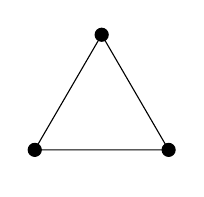
\begin{tikzpicture}[%
x={(1.7cm,0cm)},
y={(0cm,1.7cm)},
]

\coordinate (A) at (0,0); 
\coordinate (B) at (1,0) ;
\coordinate (C) at (0.5,0.86); 

%Ecken
\node[circle,scale=0.5,fill=black,draw=black](Ap) at (0,0){};
\node[circle,scale=0.5,fill=black,draw=black](Bp) at (1,0){};
\node[circle,scale=0.5,fill=black,draw=black](Cp) at (0.5,0.86){};

%Kanten
\draw[] (A)
-- (B)  node[midway, below]{}
-- (C)      node[midway, right]{}
-- (A)  node[midway, left]{};

\end{tikzpicture}
\subcaption{}
\end{minipage}
\hfill
 \begin{minipage}[t]{.2\textwidth}
   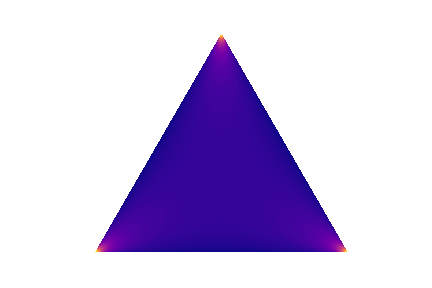
\includegraphics[width=\textwidth]{plots/notebooks/gs1.png}
\subcaption{}
\end{minipage}
\hfill
 \begin{minipage}[t]{.2\textwidth}
   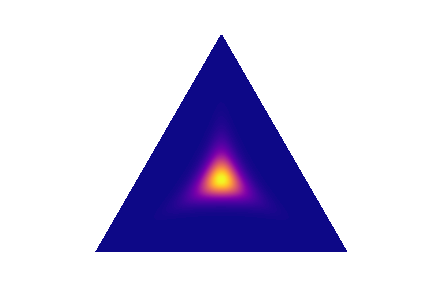
\includegraphics[width=\textwidth]{plots/notebooks/gs5.png}
\subcaption{}
\end{minipage}
\hfill
 \begin{minipage}[t]{.2\textwidth}
   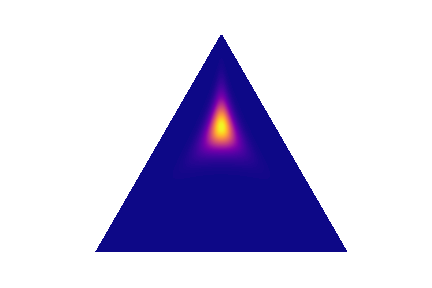
\includegraphics[width=\textwidth]{plots/notebooks/gs5_shift.png}
\subcaption{}
\end{minipage}

\caption{Пример распределения Gumbel-Softmax при различных значениях параметров: а)~$\lambda_{temp}\to0$, б)~$\lambda_{temp}=1, \mathbf{s}=[1,1,1]$, в)~$\lambda_{temp}=5, \mathbf{s}=[1,1,1]$, г)~$\lambda_{temp}=5, \mathbf{s}=[10,0.1,0.1].$}
\label{fig:gs}

\end{figure}


Заметим, что предлагаемое априорное распределение неоднозначно: одно и то же распределение  можно получить с различными значениями гиперпарамета $\mathbf{A}^{j,k}_l$ и структурного параметра $\gamma^{j,k}_l$. В качестве регуляризатора для матрицы $(\mathbf{A}^{j,k}_l)^{-1}$ предлагается использовать обратное гамма-распределение:
\[
    (\mathbf{A}^{j,k}_l)^{-1} \sim \text{inv-gamma}(\lambda_1,\lambda_2),
\]
где $\lambda_1,\lambda_2 \in \boldsymbol{\lambda}$ --- метапараметры оптимизации. 
Использование обратного гамма-распределения в качестве распределения гиперпараметров можно найти в~\cite{bishop,mackay}. В данной работе обратное распределение выступает как регуляризатор гиперпараметров.
Варьируя метапарамы $\lambda_1,\lambda_2$ получается  более сильная или более слабая регуляризация~\cite{rvm}. Пример распределений $\text{inv-gamma}(\lambda_1,\lambda_2)$ для разных значений метапараметров $\lambda_1,\lambda_2$ изображен на Рис.~\ref{fig:inv-gamma}. Оптимизации без регуляризации соответствует случай предельного распределения $\lim_{\lambda_1,\lambda_2\to 0}\text{inv-gamma}(\lambda_1, \lambda_2)$.

\begin{figure}
\centering
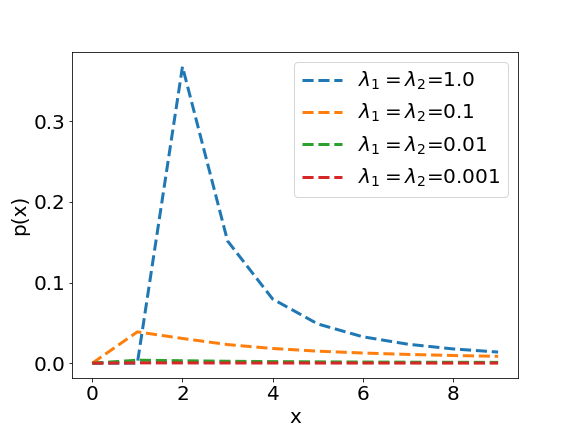
\includegraphics[width=0.6\textwidth]{plots/notebooks/invgamma.png}
\caption{Графики обратных гамма распределений для различных значений метапараметров.}
\label{fig:inv-gamma}
\end{figure}


Таким образом, предлагаемая вероятностная модель содержит следующие компоненты:
\begin{enumerate}
\item Параметры $\mathbf{w}$ модели, распределенные нормально.
\item Структура модели $\boldsymbol{\Gamma}$, содержащая все структурные параметры $\{\boldsymbol{\gamma}^{j,k}, (j,k) \in E\}$ распределены по распределению Gumbel-Softmax.
\item Гиперпараметры: $\mathbf{h} = [\text{diag}(\mathbf{A}), \mathbf{s}]$, где $\mathbf{A}$ --- конкатенация матриц $\mathbf{A}^{j,k}, (j,k) \in E,$ $\mathbf{s}$ --- конкатенация параметров Gumbel-Softmax распределений $\mathbf{s}^{j,k}, (j,k) \in E$, где $E$ --- множество ребер, соответствующих графу рассматриваемого параметрического семейства.
\item Метапараметры: $\boldsymbol{\lambda} = [\lambda_1, \lambda_2, \lambda_\text{temp}].$ Эти параметры не подлежат оптимизации и задаются экспертно. 
\end{enumerate}

График вероятностной модели в формате плоских нотаций представлен на Рис.~\ref{fig:plate_prob}.
\begin{figure}
\centering
   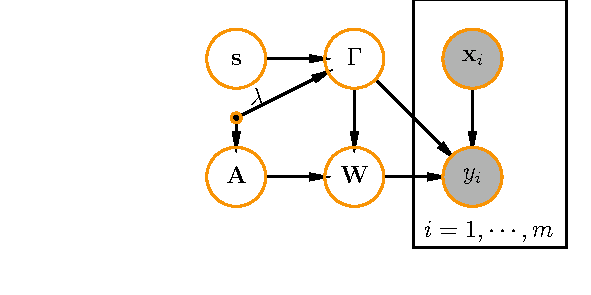
\includegraphics[width=0.5\textwidth]{plots/notebooks/simple_plate.pdf}
\caption{График предлагаемой вероятностной модели в формате плоских нотаций. Переменные обозначены белыми и серыми кругами, константы обозначены обведенными черными кругами. Наблюдаемые переменные обозначены серыми кругами.}
\label{fig:plate_prob}
\end{figure}

\section{Вариационная оценка для обоснованности вероятностной модели}
В качестве критерия выбора структуры модели предлагается использовать апостериорную вероятность гиперпараметров:
\begin{equation}
\label{eq:optimal_hyper}
    p(\mathbf{h}|\mathbf{y}, \mathbf{X}, \boldsymbol{\lambda}) \propto p(\mathbf{y}|\mathbf{X}, \mathbf{h}, \boldsymbol{\lambda}) p(\mathbf{h}|\boldsymbol{\lambda}) \to \max_{\mathbf{h} \in \mathbb{H}},
\end{equation}
где структура модели и параметры модели выбираются на основе полученных значений гиперпараметров:
\[
    \boldsymbol{\Gamma}^* = \argmax_{\boldsymbol{\Gamma} \in \amsmathbb{\Gamma}} p(\boldsymbol{\Gamma}|\mathbf{y}, \mathbf{X}, \mathbf{h}^*),
\]
\[
    \mathbf{w}^* = \argmax_{\mathbf{w} \in \mathbb{W}} p(\mathbf{w}|\mathbf{y}, \mathbf{X}, \boldsymbol{\Gamma}^*, \mathbf{h}^*),
\]
где $\mathbf{h}^*$ --- решение задачи оптимизации~\eqref{eq:optimal_hyper}.

Для вычисления обоснованности $$p(\mathbf{y}|\mathbf{X}, \mathbf{h}, \boldsymbol{\lambda}) = \iint_{\boldsymbol{\Gamma},\mathbf{w}}p(\mathbf{y}|\mathbf{X}, \mathbf{w}, \boldsymbol{\Gamma},\boldsymbol{\lambda})p(\mathbf{w}|\boldsymbol{\Gamma},\mathbf{h}, \boldsymbol{\lambda})p(\boldsymbol{\Gamma}|\mathbf{h}, \boldsymbol{\lambda})d\boldsymbol{\Gamma}d\mathbf{w}$$ из~\eqref{eq:optimal_hyper} предлагается использовать вариационную оценку обоснованности.

\begin{theorem}
Пусть $q(\mathbf{w},\boldsymbol{\Gamma}|\boldsymbol{\theta})  = q_\mathbf{w}(\mathbf{w},\boldsymbol{\Gamma}|\boldsymbol{\theta}_\mathbf{w})q_{\boldsymbol{\Gamma}}(\boldsymbol{\Gamma}|\boldsymbol{\theta}_{\boldsymbol{\Gamma}})$ --- вариационное распределение c параметрами $\boldsymbol{\theta}= [\boldsymbol{\theta}_\mathbf{w},\boldsymbol{\theta}_{\boldsymbol{\Gamma}} ]$, аппроксимирующее апостериорное распределение структуры и параметров:
\[
    q(\mathbf{w},\boldsymbol{\Gamma}|\boldsymbol{\theta}) \approx p(\mathbf{w},\boldsymbol{\Gamma}|\mathbf{y}, \mathbf{X}, \mathbf{h}, \boldsymbol{\lambda}),
\]
\[
    q_{\mathbf{w}}(\mathbf{w}|\boldsymbol{\theta}_\mathbf{w},\boldsymbol{\Gamma}) \approx p(\mathbf{w}|\mathbf{y}, \mathbf{X},  \boldsymbol{\Gamma},\mathbf{h}, \boldsymbol{\lambda}),
\]
\[
    q_{\boldsymbol{\Gamma}}(\boldsymbol{\Gamma}|\boldsymbol{\theta}_{\boldsymbol{\Gamma}}) \approx p(\boldsymbol{\Gamma}|\mathbf{y}, \mathbf{X},  \mathbf{h}, \boldsymbol{\lambda}).
\]

Тогда справедлива следующая оценка:
\begin{equation}
\label{eq:full_elbo}
\text{log} p(\mathbf{y}|\mathbf{X}, \mathbf{h}, \boldsymbol{\lambda}) \geq
\end{equation}
\[
 \mathsf{E}_{\boldsymbol{\Gamma} \sim q_{\boldsymbol{\Gamma}}}\mathsf{E}_{\mathbf{w} \sim q_{\mathbf{w}}} \text{log}p(\mathbf{y}|\mathbf{w}, \boldsymbol{\Gamma}, \mathbf{X})-D_\text{KL}\left(q_{\boldsymbol{\Gamma}}(\boldsymbol{\Gamma}|\boldsymbol{\theta}_{\boldsymbol{\Gamma}})|p(\boldsymbol{\Gamma}|\mathbf{h}, \boldsymbol{\lambda})\right) -
\]
\[
-D_\text{KL}\left(q_{\mathbf{w}}(\mathbf{w}|\boldsymbol{\theta}_\mathbf{w},\boldsymbol{\Gamma})|p(\mathbf{w}|\boldsymbol{\Gamma}, \mathbf{h})\right),
\]
где $D_\text{KL}\left(q_{\mathbf{w}}(\mathbf{w}|\boldsymbol{\theta}_\mathbf{w},\boldsymbol{\Gamma})|p(\mathbf{w}|\boldsymbol{\Gamma}, \mathbf{h})\right)$ вычисляется по формуле условной дивергенции~\cite{TODO}:
\[
D_\text{KL}\left(q_{\mathbf{w}}(\mathbf{w}|\boldsymbol{\theta}_\mathbf{w},\boldsymbol{\Gamma})|p(\mathbf{w}|\boldsymbol{\Gamma}, \mathbf{h})\right) = \mathsf{E}_{\boldsymbol{\Gamma} \sim q_{\boldsymbol{\Gamma}}} \mathsf{E}_{\mathbf{w} \sim q_{\mathbf{w}}} \text{log}\left(\frac{q(\mathbf{w}|\boldsymbol{\Gamma})}{p(\mathbf{w}|\mathbf{h},\boldsymbol{\Gamma})}\right).
\]
\end{theorem}

\begin{proof}
Рассмотрим обоснованность:
\[
text{log}~p(\mathbf{y}|\mathbf{X}, \mathbf{h}, \boldsymbol{\lambda}) =  \text{log}~\iint_{\boldsymbol{\Gamma},\mathbf{w}}p(\mathbf{y}|\mathbf{X}, \mathbf{w}, \boldsymbol{\Gamma},\boldsymbol{\lambda})p(\mathbf{w}|\boldsymbol{\Gamma},\mathbf{h}, \boldsymbol{\lambda})p(\boldsymbol{\Gamma}|\mathbf{h}, \boldsymbol{\lambda})d\boldsymbol{\Gamma}d\mathbf{w}  =
\]
\[
  =   \text{log}~\iint_{\boldsymbol{\Gamma},\mathbf{w}} p(\mathbf{y}|\mathbf{X}, \mathbf{w}, \boldsymbol{\Gamma},\boldsymbol{\lambda})p(\mathbf{w}|\boldsymbol{\Gamma},\mathbf{h}, \boldsymbol{\lambda})p(\boldsymbol{\Gamma}|\mathbf{h}, \boldsymbol{\lambda})\frac{q(\mathbf{w}, \boldsymbol{\Gamma}|\boldsymbol{\theta})}{q(\mathbf{w}, \boldsymbol{\Gamma}|\boldsymbol{\theta})}d\boldsymbol{\Gamma}d\mathbf{w} =
\]
\[
  =  \text{log} \mathsf{E}_q \frac{p(\mathbf{y}|\mathbf{X}, \mathbf{h}, \boldsymbol{\lambda})}{q(\mathbf{w}, \boldsymbol{\Gamma}|\boldsymbol{\theta})}.
\]
Используя неравенство Йенсена получим 
\[
 \text{log} \mathsf{E}_q \frac{p(\mathbf{y}|\mathbf{X}, \mathbf{h}, \boldsymbol{\lambda})}{q(\mathbf{w}, \boldsymbol{\Gamma}|\boldsymbol{\theta})}     \geq  \mathsf{E}_q\text{log}~\frac{p(\mathbf{y}|\mathbf{X}, \mathbf{h}, \boldsymbol{\lambda})}{q(\mathbf{w}, \boldsymbol{\Gamma}|\boldsymbol{\theta})} =
\]
\[
   \mathsf{E}_{q} \text{log}p(\mathbf{y}|\mathbf{w}, \boldsymbol{\Gamma}, \mathbf{X})-D_\text{KL}(q (\mathbf{w},\boldsymbol{\Gamma}|\boldsymbol{\theta})|p(\mathbf{w},\boldsymbol{\Gamma}|\mathbf{h}, \boldsymbol{\lambda})).
\]
Декомпозируем распределение $q$ по свойству условной дивергенции:
\[
D_\text{KL}(q (\mathbf{w},\boldsymbol{\Gamma}|\boldsymbol{\theta})|p(\mathbf{w},\boldsymbol{\Gamma}|\mathbf{h})) = 
\]
\[
=D_\text{KL}\left(q_{\boldsymbol{\Gamma}}(\boldsymbol{\Gamma}|\boldsymbol{\theta}_{\boldsymbol{\Gamma}})|p(\boldsymbol{\Gamma}|\mathbf{h}, \boldsymbol{\lambda})\right)+D_\text{KL}\left(q_{\mathbf{w}}(\mathbf{w}|\boldsymbol{\theta}_\mathbf{w},\boldsymbol{\Gamma})|p(\mathbf{w}|\boldsymbol{\Gamma}, \mathbf{h}, \boldsymbol{\lambda})\right).    
\]
\end{proof}
В качестве вариационного распределения $q_{\mathbf{w}}$ предлагается использовать нормальное распределение, не зависящее от структуры модели $\boldsymbol{\Gamma}$:
\[
    q_{\mathbf{w}} = \mathcal{N}(\boldsymbol{\mu}_q, \mathbf{A}_q), 
\]
где $\mathbf{A}_q$ --- диагональная матрица с диагональю $\boldsymbol{\alpha}_q$.

В качестве вариационного распределения $q_{\boldsymbol{\Gamma}}$ предлагается использовать произведение распределений Gumbel-Softmax. Конкатенацию параметров концентрации распределений обозначим $\mathbf{s}_q$. Его температуру, общую для всех структурных параметров $\boldsymbol{\gamma} \in \boldsymbol{\Gamma}$, обозначим $\theta_\text{temp}$.
Вариационными параметрами распределения $q$ являются параметры распределений $q_{\mathbf{w}}, q_{\boldsymbol{\Gamma}}$:
\[\boldsymbol{\theta}=[\boldsymbol{\mu}_q, \boldsymbol{\alpha}_q,\mathbf{s}_q, \theta_\text{temp}]. 
\]
График вероятностной вариационной модели в формате плоских нотаций представлен на Рис.~\ref{fig:plate_qprob}.
\begin{figure}
\centering
   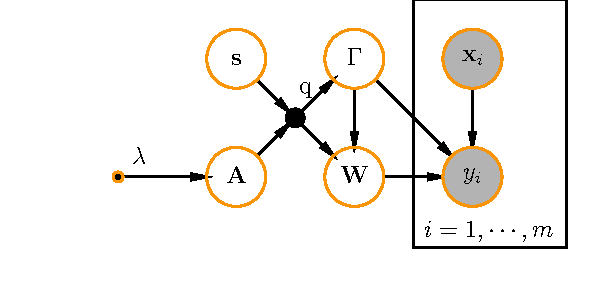
\includegraphics[width=0.5\textwidth]{plots/notebooks/plate.pdf}
\caption{График предлагаемой вероятностной вариационной модели в формате плоских нотаций. Переменные обозначены белыми и серыми кругами, константы обозначены обведенными черными кругами. Вариационное распределение обозначено черным кругом. Наблюдаемые переменные обозначены серыми кругами.}
\label{fig:plate_qprob}
\end{figure}

Для анализа сложности полученной модели введем понятие \textit{параметрической сложности}. 
\begin{defin} 
Параметрической сложностью  $C_p(\boldsymbol{\theta}|U_\mathbf{h},\boldsymbol{\lambda})$ модели с вариационными параметрами $\boldsymbol{\theta}$ на компакте $U_\mathbf{h} \subset \mathbb{H}$ назовем минимальную дивергенцию между вариационным и априорным распределением:
\[
C_p(\boldsymbol{\theta}|U_\mathbf{h},\boldsymbol{\lambda}) = \min_{\mathbf{h} \in U_\mathbf{h}} \text{D}_\text{KL}\left(q(\mathbf{w}, \boldsymbol{\Gamma}|\boldsymbol{\theta})|p(\mathbf{w}, \boldsymbol{\Gamma}|\mathbf{h},\boldsymbol{\lambda})\right).
\]
\end{defin}
Параметрическая сложность модели соответствует ожидаемой длине описания параметров модели при условии заданного параметрического априорного распределения~\cite{hinton_mdl}.

Одним из критериев удаления неинформативных параметров в вероятностных моделях является отношение вариационной плотности параметров в моде распределения к вариационной плотности параметра в нуле~\cite{nips}:
\[\frac{q_\mathbf{w}(w=\mu_q|\boldsymbol{\theta}_\mathbf{w})}{q_\mathbf{w}(w=0|\boldsymbol{\theta}_\mathbf{w})}= \text{exp}\left(-\frac{2\alpha_q^2}{\mu_q^2}\right),
\]
где $q_\mathbf{w}(w|\boldsymbol{\theta}_\mathbf{w}) \sim \mathcal{N}(\mu_q, \alpha_q).$

Обобщим понятие относительной вариационной плотности на случай произвольных непрерывных распределений.
\begin{defin}
Относительной вариационной   плотностью параметра $w \in \mathbf{w}$  при условии структуры $\boldsymbol{\Gamma}$ и гиперпараметров $\mathbf{h}$ назовем отношение вариационной плотности в моде вариационного распределения параметра к вариационной плотности в моде априорного распределению параметра:
\[\rho(w|\boldsymbol{\Gamma},\boldsymbol{\theta}_\mathbf{w}, \mathbf{h},\boldsymbol{\lambda})=\frac{q\bigl(\text{mode}~q\left(w|\boldsymbol{\Gamma}, \boldsymbol{\theta}_\mathbf{w}\right)|\boldsymbol{\Gamma}, \boldsymbol{\theta}_\mathbf{w}\bigr)}{q\bigl(\text{mode}~p\left({w}|\boldsymbol{\Gamma}, \mathbf{h},\boldsymbol{\lambda}\right)|\boldsymbol{\Gamma},\boldsymbol{\theta}_\mathbf{w}\bigr)}.\]
Относительной вариационной плотностью вектора параметров $\mathbf{w}$ назовем следующее выражение:
\[
    \boldsymbol{\rho}(\mathbf{w}|\boldsymbol{\Gamma}, \boldsymbol{\theta}_\mathbf{w}, \mathbf{h},\boldsymbol{\lambda}) = \prod_{w \in \mathbf{w}}\rho(w|\boldsymbol{\Gamma}, \boldsymbol{\theta}_\mathbf{w}, \mathbf{h},\boldsymbol{\lambda}).
\]

\end{defin}

Сформулируем и докажеми теорему о связи относительной плотности и параметрической сложности модели:

\begin{theorem}
Пусть
\begin{enumerate}
\item заданы компактные множества $U_\mathbf{h} \subset \mathbb{H}, U_{\boldsymbol{\theta}_\mathbf{w}} \times U_{\boldsymbol{\theta}_{\boldsymbol{\Gamma}}} \subset \amsmathbb{\Theta}$;


\item Мода априорного распределения $p(\mathbf{w},\boldsymbol{\Gamma}| \mathbf{h}, \boldsymbol{\lambda})$ не зависит от гиперпараметров $\mathbf{h}$  на $U_\mathbf{h}$ и структуры $\boldsymbol{\Gamma}$ на $U_{\boldsymbol{\theta}_{\boldsymbol{\Gamma}}}$:
\[\text{mode}~p(\mathbf{w}|\boldsymbol{\Gamma}_1, \mathbf{h}_1, \boldsymbol{\lambda})=\text{mode}~ p(\mathbf{w}|\boldsymbol{\Gamma}_2,\mathbf{h}_2, \boldsymbol{\lambda})=\mathbf{M}~\forall~\mathbf{h}_1, \mathbf{h}_2\in U_\mathbf{h},\boldsymbol{\Gamma}_1, \boldsymbol{\Gamma}_2\in U_{\boldsymbol{\theta}_{\boldsymbol{\Gamma}}}.
\]

\item вариационное распределение $q_\mathbf{w}$ и априорное распределение $p(\mathbf{w}|\boldsymbol{\Gamma}, \mathbf{h})$  являются абсолютно непрерывными и унимодальными на  $U_\mathbf{h}, U_{\boldsymbol{\theta}}$.

\item Параметры модели $\mathbf{w}$ имеют конечные вторые моменты по распределениям $q(\mathbf{w}, \boldsymbol{\Gamma}|\boldsymbol{\theta}), p(\mathbf{w}, \boldsymbol{\Gamma}|\mathbf{h}, \boldsymbol{\lambda})$:
\[
    \mathsf{E}_q \mathbf{w}^2 = \mathsf{E}_{q_{\boldsymbol{\Gamma}}}\mathsf{E}_{q_\mathbf{w}}\mathbf{w}^2 < \infty;
\]
\[
    \mathsf{E}_{p(\mathbf{w},\boldsymbol{\Gamma}|\mathbf{h}, \boldsymbol{\lambda})}\mathbf{w}^2 = \mathsf{E}_{p(\boldsymbol{\Gamma}|\mathbf{h}, \boldsymbol{\lambda})} \mathsf{E}_{p(\mathbf{w}|\boldsymbol{\Gamma}, \mathbf{h}, \boldsymbol{\lambda})}\mathbf{w}^2 < \infty;
\]

\item мода и матожидание вариационного распределения $q_\mathbf{w}$ и априорного распределения $p(\mathbf{w}|\boldsymbol{\Gamma},\mathbf{h}, \boldsymbol{\lambda})$  совпадают:
\[
    \text{mode}~p(\mathbf{w}|\boldsymbol{\Gamma},\mathbf{h}, \boldsymbol{\lambda}) = \mathsf{E}_{p(\mathbf{w}| \boldsymbol{\Gamma}, \mathbf{h}, \boldsymbol{\lambda})} \mathbf{w};
\]
\[
  \text{mode}~q(\mathbf{w}|\boldsymbol{\Gamma}, \boldsymbol{\theta}_\mathbf{w}) = \mathsf{E}_{q_\mathbf{w}(\mathbf{w}|\boldsymbol{\Gamma},  \boldsymbol{\theta}_\mathbf{w})} \mathbf{w};
\]

\item задана  бесконечная последовательность векторов вариационных параметров $\boldsymbol{\theta}_1,\boldsymbol{\theta}_2,\dots, \boldsymbol{\theta}_i \in U_{\boldsymbol{\theta}}$, такая что $\lim_{i \to \infty}C_p(\boldsymbol{\theta_i}|U_{\mathbf{h}}, \boldsymbol{\lambda}) = 0.$ 

\end{enumerate}
Тогда следующее выражение стремится к единице:
\[
   \mathsf{E}_{q_{\boldsymbol{\Gamma}}} \boldsymbol{\rho}(\mathbf{w}|\boldsymbol{\Gamma}, \boldsymbol{\theta}_\mathbf{w}, \mathbf{h},\boldsymbol{\lambda})^{-1} \to 1.
\]


\end{theorem}

\begin{proof}
Воспользуемся неравенством Пинскера:
\[
    ||F_q(\boldsymbol{\theta})-F_p(\mathbf{h})||_\text{TV},\leq\sqrt{2\text{D}_\text{KL}\left(q(\mathbf{w}, \boldsymbol{\Gamma}|\boldsymbol{\theta})|p(\mathbf{w}, \boldsymbol{\Gamma}|\mathbf{h})\right)},
\]
где $||\cdot||_\text{TV}$ --- расстояние по вариации, $F_q, F_p$ --- функции распределения   $q(\mathbf{w},\boldsymbol{\Gamma}|\boldsymbol{\theta})$ и $p(\mathbf{w},\boldsymbol{\Gamma}| \mathbf{h}, \boldsymbol{\lambda})$.
Отсюда $ \lim_{i \to \infty} ||F_q(\boldsymbol{\theta})-F_p(\mathbf{h})||_\text{TV} = 0.$
Из сходимости по вариации следует слабая сходимость распределений.
Рассмотрим разность усредненных мод:
\[
|\mathsf{E}_{q_{\boldsymbol{\Gamma}}}\text{mode}~q_{\mathbf{w}}(\mathbf{w}|\boldsymbol{\theta}_\mathbf{w},\boldsymbol{\Gamma})-\mathsf{E}_{p(\boldsymbol{\Gamma}|\mathbf{h}, \boldsymbol{\lambda})} \text{mode}~p(\mathbf{w}|\boldsymbol{\Gamma}, \mathbf{h})| = 
\]
\[
=|\mathsf{E}_{q_{\boldsymbol{\Gamma}}} \mathsf{E}_{q_\mathbf{w}} \mathbf{w}-\mathsf{E}_{p(\boldsymbol{\Gamma}|\mathbf{h}, \boldsymbol{\lambda})} \mathsf{E}_{p(\mathbf{w}| \boldsymbol{\Gamma}, \mathbf{h}, \boldsymbol{\lambda})} \mathbf{w}| =
\]
\[
= |\mathsf{E}_{q}\mathbf{w}-\mathsf{E}_{p(\mathbf{w},\boldsymbol{\Gamma}|\mathbf{h})}\mathbf{w}|.
\]
Т.к. вторые моменты величины $\mathbf{w}$ конечны для вариационного и априорного распределения, то функции $\mathsf{E}_{q}\mathbf{w}, \mathsf{E}_{p(\mathbf{w},\boldsymbol{\Gamma}| \mathbf{h})}\mathbf{w}$ равномерно интегрируемы. Если случайные величиные слабо сходятся и являются равномерно интегрируемыми, то существует сходимость в среднем, предел выражения можно поставить под знак интеграла:
\[
  \lim_{i \to \infty}\bigl( |\mathsf{E}_{q}\mathbf{w}- \mathsf{E}_{p(\mathbf{w},\boldsymbol{\Gamma}|\mathbf{h})}\mathbf{w}| \bigr) \leq    \lim_{i \to \infty}\bigl( \mathsf{E}_{\mathbf{w}_1 \sim q, \mathbf{w}_2 \sim p(\mathbf{w},\boldsymbol{\Gamma}|\mathbf{h})}|\mathbf{w}_1- \mathbf{w}_2| \bigr) =0.
\]
Т.к. вторые моменты случайных величин конечны, то конечны и первые моменты:
\[
  \lim_{i \to \infty} \mathsf{E}_{q}\mathbf{w}= \lim_{i \to \infty}\mathsf{E}_{p(\mathbf{w},\boldsymbol{\Gamma}|\mathbf{h})}\mathbf{w} = \mathbf{M}.
\]
Таким образом в пределе усредненные по структуре моды вариационного распределения $q_\mathbf{w}(\mathbf{w}|\boldsymbol{\Gamma}, \boldsymbol{\theta})$ и априорного распределения $p(\mathbf{w}|\boldsymbol{\Gamma}, \mathbf{h})$ совпадают.
%http://www.math.chalmers.se/~serik/WeakConv/C-space.pdf
%https://math.stackexchange.com/questions/2923/do-convergence-in-distribution-along-with-uniform-integrability-imply-convergenc
% https://web.ma.utexas.edu/users/gordanz/notes/uniform_integrability.pdf   
%file:///home/legin/%D0%97%D0%B0%D0%B3%D1%80%D1%83%D0%B7%D0%BA%D0%B8/weak_convergence.pdf
Т.к. наибольшее значение распределения $q_\mathbf{w}$ сосредоточено в моде распределения $q_\mathbf{w}$, то $\boldsymbol{\rho}(\mathbf{w}|\boldsymbol{\Gamma}, \boldsymbol{\theta}_\mathbf{w}, \mathbf{h},\boldsymbol{\lambda})^{-1}$ ограничена сверху единицей. Рассмотрим матожидание функции, обратной к отношению вариационных плотностей:
\[
\mathsf{E}_q \boldsymbol{\rho}(\mathbf{w}|\boldsymbol{\Gamma}, \boldsymbol{\theta}_\mathbf{w}, \mathbf{h},\boldsymbol{\lambda})^{-1}
\] 
Т.к. функция $\boldsymbol{\rho}(\mathbf{w}|\boldsymbol{\Gamma}, \boldsymbol{\theta}_\mathbf{w}, \mathbf{h},\boldsymbol{\lambda})^{-1}$  ограничена, то предел можно внести под знак интеграла:
\[
\lim_{i \to \infty} \mathsf{E}_q \boldsymbol{\rho}(\mathbf{w}|\boldsymbol{\Gamma}, \boldsymbol{\theta}_\mathbf{w}, \mathbf{h},\boldsymbol{\lambda})^{-1} = 
 \mathsf{E}_q  \lim_{i \to \infty}  \boldsymbol{\rho}(\mathbf{w}|\boldsymbol{\Gamma}, \boldsymbol{\theta}_\mathbf{w}, \mathbf{h},\boldsymbol{\lambda})^{-1} =
\]
\[
    \mathsf{E}_q \lim_{i \to \infty} \prod_{w \in \mathbf{w}}\frac{q\bigl(\text{mode}~p\left({w}|\boldsymbol{\Gamma}, \mathbf{h},\boldsymbol{\lambda}\right)|\boldsymbol{\Gamma},\boldsymbol{\theta}_\mathbf{w}\bigr)}{q\bigl(\text{mode}~q\left(w|\boldsymbol{\Gamma}, \boldsymbol{\theta}_\mathbf{w}\right)|\boldsymbol{\Gamma}, \boldsymbol{\theta}_\mathbf{w}\bigr)}=
\]
\[
     \mathsf{E}_q \frac{q_\mathbf{w}(\mathbf{M})}{q_\mathbf{w}(\mathbf{M})} = 1.
\]
Заметим, что $ \mathsf{E}_q \frac{q_\mathbf{w}(\mathbf{M})}{q_\mathbf{w}(\mathbf{M})} = \mathsf{E}_{q_{\boldsymbol{\Gamma}}}\frac{q_\mathbf{w}(\mathbf{M})}{q_\mathbf{w}(\mathbf{M})}$ и получим итоговый результат.
\end{proof}

Теорема утверждает, что при устремлении параметрической сложности модели к нулю, все параметры модели подлежат удалению в среднем по всем возможным значениям  структуры $\boldsymbol{\Gamma}$ модели. Заметим, что теорема применима для случая, когда последовательность вариационных распределений $q$ не имеет предела. Так, в случае, если структура $\boldsymbol{\Gamma}$ определена однозначно, последовательность $q_i$ может являться последовательностью нормальных распределений, чье матожидание стремится к нулю:
\[
    q_i \sim \mathcal{N}((\boldsymbol{\mu}_q)_i, (\mathbf{A}^{-1}_q)_i), (\boldsymbol{\mu}_q)_i \to \mathbf{0}.
\]
Априорным распределением $p(\mathbf{w},\boldsymbol{\Gamma}|\mathbf{h},\boldsymbol{\lambda}) = p(\mathbf{w}|\mathbf{h},\boldsymbol{\lambda})$ при этом может являться семейство нормальных распределений с нулевым средним:
\[
    p(\mathbf{w}|\mathbf{h},\boldsymbol{\lambda}) = \mathcal{N}(\mathbf{0}, \mathbf{A}^{-1}).
\]
При этом сама последовательность распределений $q_i$ не обязана иметь предел.

\section{Обобщающая задача}
В данном разделе проводится анализ основных критериев выбора моделей, а также предлагается их обобщение на случай моделей, испольюзующих вариационное распределение $q$ для аппроксимации неизвестного апостериорного распределения параметров $p(\mathbf{w}, \boldsymbol{\Gamma}|\mathbf{y}, \mathbf{X}, \mathbf{h}, \boldsymbol{\lambda})$.

Рассмотрим основные статистические критерии выбора вероятностных моделей. 
\begin{enumerate}
\item Критерий максимального правдоподобия:
\[\text{log}p(\mathbf{y}|\mathbf{X},\mathbf{w}, \boldsymbol{\Gamma})\to \max_{\mathbf{w}\in \mathbb{W}, \boldsymbol{\Gamma}\in \amsmathbb{\Gamma}}.\]

Метод заключается в максимизации правдоподобия выборки и подвержен переобучению.
Для использования данного метода в качестве задачи выбора модели предлагается следующее обобщение:
\begin{equation}
\label{eq:optim_ml}
    L =  \mathsf{E}_q \text{log}~p(\mathbf{y}|\mathbf{X}, \mathbf{w}, \boldsymbol{\Gamma}).
\end{equation}
Данное обобщение~\eqref{eq:optim_ml} эквивалентно  критерию правдоподобия при выборе в качестве $q$ эмпирического распределения парамтетров и структуры.
Метод не предполагает оптимизации гиперпараметров $\mathbf{h}$. Для формального соответствия данной задачи задаче выбора модели~\eqref{TOD}, т.е. двухуровневой задачи оптимизации, положим $L=Q:$
\[
    L =  \mathsf{E}_q \text{log}~p(\mathbf{y}|\mathbf{X}, \mathbf{w}, \boldsymbol{\Gamma}) \to \max_{\boldsymbol{\theta}},
\]
\[
    Q =  \mathsf{E}_q \text{log}~p(\mathbf{y}|\mathbf{X}, \mathbf{w}, \boldsymbol{\Gamma}).
\]



\item Метод максимальной апостериорной вероятности. 
\[\text{log}~p(\mathbf{y},\mathbf{w},\boldsymbol{\Gamma}|\mathbf{X}, \boldsymbol{\lambda} )\to \max_{\mathbf{w} \in \mathbb{W}, \boldsymbol{\Gamma}\in \amsmathbb{\Gamma}}.\]
Аналогично предыдущему методу сформулируем вариационное обобщение данной задачи:
\begin{equation}
\label{eq:optim_map}
L=Q =\mathsf{E}_q\bigl(\text{log}~p(\mathbf{y}|\mathbf{X}, \mathbf{w},\boldsymbol{\Gamma})+\text{log}p(\mathbf{w}, \boldsymbol{\Gamma}|\boldsymbol{\lambda}).
\end{equation}
Т.к. в рамках данной задачи~\eqref{eq:optim_map} не предполагается оптимизации гиперпараметров $\mathbf{h}$, положим параметры распределения $p(\mathbf{w}, \boldsymbol{\Gamma}|\mathbf{h}, \boldsymbol{\lambda})$ фиксированными:
\[
    \boldsymbol{\lambda} = [\lambda_1, \lambda_2, \lambda_{\text{temp}}, \mathbf{s}, \text{diag}(\mathbf{A})].
\]

\item Перебор структуры:
\begin{equation}
\label{eq:optim_struct}
    L =  Q = \mathsf{E}_q\text{log}p(\mathbf{y}, \mathbf{w}|\mathbf{X})[q_{\boldsymbol{\Gamma}} = p']
\end{equation}
где $p'$ --- некоторое распределение на структуре $\boldsymbol{\Gamma}$, выступающее в качестве метапараметра.




\item Критерий Акаике:
\[
   \text{AIC} =  \text{log}p(\mathbf{y}|\mathbf{X}, \mathbf{w}, \boldsymbol{\Gamma})-|\mathbb{W}|.
\]
Т.к. все рассматриваемые модели принадлежат одному параметрическому семейству моделей $\mathfrak{F}$, то количество параметров у всех рассматриваемых моделей  совпадает . Тогда критерий Акаике совпадает с критерием максимального правдоподобия. Для использования критерия Акаике для сравнения моделей, принадлежащих одному параметрическому семейству~$\mathfrak{F}$ предлагается следующая переформулировка:
\begin{equation}
\label{eq:optim_aic}
    L = Q = \text{log}p(\mathbf{y}|\mathbf{X}, \mathbf{w}, \boldsymbol{\Gamma})
-|\{w: D_\text{KL}(\theta, \mathbf{h})<\lambda_{\text{prune}}\}|,
\end{equation}
где 
\begin{equation}\label{eq:aic_compl}\mathbf{h}=\argmin_{\mathbf{h}'\in U_\mathbf{h}}D_\text{KL}(q(\mathbf{w},\boldsymbol{\Gamma})| p(\mathbf{w},\boldsymbol{\Gamma}|\mathbf{h}',\boldsymbol{\lambda}),\end{equation} $\lambda_{\text{prune}}$ --- метапараметр алгоритма, $U_\mathbf{h}  \subset \mathbb{H}$ --- область определения задачи по гиперпараметрам. Предложенное обобщение~\eqref{eq:optim_aic} применимо только в случае, если выражение~\eqref{eq:aic_compl} определено однозначно, т.е. существует единственный вектор гиперпараметров на $U_\mathbf{h},$ доставляющий минимум дивергенции $D_\text{KL}(q(\mathbf{w},\boldsymbol{\Gamma})| p(\mathbf{w},\boldsymbol{\Gamma}|\mathbf{h},\boldsymbol{\lambda}).$

\item Информационный критерий Шварца:
\[
    \text{BIC} = \text{log}p(\mathbf{y}|\mathbf{X}, \mathbf{w})-0.5\text{log}(m)|\mathbb{W}|.
\]
Переформулируем данный критерий аналогично критерию AIC:
\begin{equation}
\label{eq:optim_bic}
    L = Q = BIC_{\lambda} = \text{log}p(\mathbf{y}|\mathbf{X}, \mathbf{w}) - \text{log}(m)|\{w: D_\text{KL}(\theta, \mathbf{h})<\lambda_{\text{prune}}\}|,
\end{equation}
метапараметр $\lambda_{\text{prune}}$ определен аналогично~\eqref{eq:aic_compl}.

\item Метод вариационной оценки обоснованности:
\begin{equation}
\label{eq:optim_elbo_method}   
    L = \mathsf{E}_q \text{log}p(\mathbf{y}|\mathbf{X}, \mathbf{w}, \boldsymbol{\Gamma})-D_\text{KL}(q(\mathbf{w}, \boldsymbol{\Gamma}|\boldsymbol{\theta})|p(\boldsymbol{\Gamma}, \mathbf{w}|\mathbf{h},\boldsymbol{\lambda}))  + \text{log}~p(\mathbf{h}|\boldsymbol{\lambda}) \to \max_{\boldsymbol{\theta}},
\end{equation}
\[
    Q = \mathsf{E}_q \text{log}p(\mathbf{y}|\mathbf{X}, \mathbf{w}, \boldsymbol{\Gamma})-D_\text{KL}(q(\mathbf{w}, \boldsymbol{\Gamma}|\boldsymbol{\theta})|p(\boldsymbol{\Gamma}, \mathbf{w}|\mathbf{h},\boldsymbol{\lambda}))  + \text{log}~p(\mathbf{h}|\boldsymbol{\lambda}) \to \max_{\mathbf{h}},
\]
В рамках данной задачи функции $L$ и $Q$ совпадают, все гиперпараметры $\mathbf{h}$ подлежат оптимизации.

\item Валидация на отложенной выборке:
\begin{equation}
\label{eq:optim_hold_out}
    L = \mathsf{E}_q \text{log}p(\mathbf{y}_\text{train}, \mathbf{w}, \boldsymbol{\Gamma}|\mathbf{X}_\text{train}, \mathbf{h}, \boldsymbol{\lambda}) \to \max_{\boldsymbol{\theta}},
\end{equation}
\[
    Q = \mathsf{E}_q \text{log}p(\mathbf{y}_\text{test}|\mathbf{X}_\text{test}, \mathbf{w}, \boldsymbol{\Gamma}) \to \max_{\mathbf{h}},
\]
где $(\mathbf{X}_\text{train}, \mathbf{y}_\text{train}), (\mathbf{X}_\text{test}, \mathbf{y}_\text{test})$ --- разбиение выборки на обучающую и контрольную подвыборку.
В рамках данной задачи, все гиперпараметры $\mathbf{h}$ подлежат оптимизации.

\end{enumerate}

Каждый из рассмотренных критерии удовлетворяет хотя бы одному из перечисленных свойств:
\begin{enumerate}[label={\arabic*)}]
\item модель, оптимизируемая согласно критерию, доставляет максимум правдоподобия выборки;
\item модель, оптимизируемая согласно критерию, доставляет максимум оценки обоснованности;
\item для моделей, доставляющих сопоставимые значения правдоподобия выборки, выбирается модель с меньшим количеством информативных параметров.
\item критерий позволяет производить перебор структур для отбора наилучших модели.
\end{enumerate}

Формализуем рассмотренные критерии. Оптимизационную задачу, которая удовлетворяет всем перечисленным свойствам при некоторых значинях метапараметров, будет называть \textit{обобщающей}.

\begin{defin}
Двухуровневую задачу оптимизации будем называть \textit{обобщающей} на компакте $U = U_{\boldsymbol{\theta}} \times U_{\mathbf{h}} \times U_{\boldsymbol{\lambda}} \subset \amsmathbb{\Theta} \times \mathbb{H} \times \amsmathbb{\Lambda}$, если она удовлетворяет следующим критериям.
\begin{enumerate}
\item Область определения каждого параметра $w \in \mathbf{w}$, гиперпараметра $h \in \mathbf{h}$ и метапараметра $\lambda \in \boldsymbol{\lambda}$ не  является пустым множеством и не является точкой.
\item Для каждого значения гиперпараметров $\mathbf{h}$ оптимальное решение нижней~\eqref{TODO} задачи оптимизации $\boldsymbol{\theta}^{*}$ определено однозначно при любых значениях метапараметров $\boldsymbol{\lambda} \in U_{\lambda}$.

\item Критерий максимизации правдоподобия выборки: существует $\boldsymbol{\lambda} \in U_{\lambda}$ и  $$K_1>0, K_1 < \max_{\mathbf{h}_1, \mathbf{h}_2 \in U_\mathbf{h}} Q(\mathbf{h}_1) - Q(\mathbf{h}_2),$$ такие что для любых векторов гиперпараметров, удовлетворяющих неравенству $$\mathbf{h}_1, \mathbf{h}_2 \in U_{h}, Q(\mathbf{h}_1)-Q(\mathbf{h}_2) > K_1,$$ выполняется неравенство $$\mathsf{E}_q \text{log}~p(\mathbf{y}|\mathbf{X}, \boldsymbol{\theta}^{*}(\mathbf{h}_1), \lambda_{\text{temp}}, \mathbf{f})>\mathsf{E}_q \text{log}~p(\mathbf{y}|\mathbf{X}, \boldsymbol{\theta}^{*}(\mathbf{h}_2), \lambda_{\text{temp}}, \mathbf{f}).$$

\item Критерий минимизации параметрической сложности:  существует  $\boldsymbol{\lambda} \in U_{\lambda}$ и $$K_2>0,K_2 < \max_{\mathbf{h}_1, \mathbf{h}_2 \in U_\mathbf{h}} Q(\mathbf{h}_1) - Q(\mathbf{h}_2),$$  такие что для любых векторов гиперпараметров $\mathbf{h}_1, \mathbf{h}_2 \in U_\mathbf{h}$, удовлетворяющих неравенству $$Q(\mathbf{h}_1)-Q(\mathbf{h}_2) > K_2,$$ параметрическая сложность первой модели меньше, чем второй: $$C_p(\boldsymbol{\theta}^{*}(\mathbf{h}_1)|U_\mathbf{h},\boldsymbol{\lambda})<C_p(\boldsymbol{\theta}^{*}(\mathbf{h}_2)|U_\mathbf{h},\boldsymbol{\lambda}).$$

\item Критерий приближения оценки обоснованности: существует значение гиперпараметров $\boldsymbol{\lambda}$, такое что значение функций потерь $L$ и валидации $Q$ пропорционален вариационной оценки обоснованности модели: $$Q \propto  L \propto 
\mathsf{E}_q p(\mathbf{y}|\mathbf{w}, \mathbf{X})-{D}_{KL}(q(\mathbf{w}, \boldsymbol{\Gamma}|\boldsymbol{\theta})|p(\mathbf{w}, \boldsymbol{\Gamma}|\mathbf{h}, \boldsymbol{\lambda}) + \text{log}~p(\mathbf{h}|\boldsymbol{\lambda})).
$$ для всех $\boldsymbol{\theta}\in U_{\boldsymbol{\theta}}, \mathbf{h} \in U_{\mathbf{h}}.$ 

\item Критерий перебора оптимальных структур: существует набор метапараметров $\boldsymbol{\lambda}$ и константа $$K_3>0, K_3 < \max_{\mathbf{h}_1, \mathbf{h}_2} D_\text{KL}(p (\boldsymbol{\Gamma}|\mathbf{h}_1, \boldsymbol{\lambda}) | p (\boldsymbol{\Gamma}|\mathbf{h}_2, \boldsymbol{\lambda})),$$ такие что для локальных оптимумов задачи оптимизации $\mathbf{h}_{1}, \mathbf{h}_2$, полученных при метапараметрах $\lambda$ и удовлетворяющих неравенствам $$D_\text{KL}(p (\boldsymbol{\Gamma}|\mathbf{h}_1, \boldsymbol{\lambda})| p (\boldsymbol{\Gamma}|\mathbf{h}_2, \boldsymbol{\lambda})) > K_3, p(\boldsymbol{\Gamma}|\mathbf{h}_2, \boldsymbol{\lambda})| p(\boldsymbol{\Gamma}|\mathbf{h}_1, \boldsymbol{\lambda})) > K_3,$$ $$Q(\mathbf{h}_1) > Q(\mathbf{h}_2),$$  существует значение метапараметров $\boldsymbol{\lambda}'$, такие что
\begin{enumerate}
\item Соответствие между вариационными параметрами $\boldsymbol{\theta}^{*}(\mathbf{h}_1), \boldsymbol{\theta}^{*}(\mathbf{h}_2)$ сохраняется при  $\boldsymbol{\lambda}'$.
\item  $Q(\mathbf{h}_1) < Q(\mathbf{h}_2)$ при $\boldsymbol{\lambda}'$.
\end{enumerate}


\item Критерий нерперывности: функции $L$ и $Q$ непрерывны по метапараметрам $\boldsymbol{\lambda} \in U_{\boldsymbol{\lambda}}$.
\end{enumerate}
\end{defin}
Первый критерий является техническим и используется для исключения из рассмотрения вырожденных задач оптимизации.  
Второй критерий говорит о том, что решение первого и второго уровня должны быть согласованы и определены однозначно.
Критерии 3-5 определяют возможные критерии оптимизации, которые должны приближаться обобщающей задачей.
Критерий 6 говорит о возможности перехода между различными структурами модели. Отметим, что данное условие крайне важно в условиях оптимизации моделей глубокого обучения, которые отличаются многоэкстремальностью. Отметим также, что данный критерий говорит о том, что мы можем перейти от одного набора гиперпараметров $\mathbf{h}_1$ к другим $\mathbf{h}_2$, если они соответствуют локальным оптимумам задачи оптимизации и дивергенция соответствующих априорных  распределений на структурах $p(\boldsymbol{\Gamma}|\mathbf{s}, \lambda_\text{temp}).$ При этом соответствующие вариационные распределения $q(\boldsymbol{\Gamma}|\boldsymbol{\theta}_{\boldsymbol{\Gamma}})$ могут оказаться достаточно близки. Возможным дополнением этого критерия был бы критерий, позволяющий переходить от структуры к структуре, если соответствующие распределения $q(\boldsymbol{\Gamma}|\boldsymbol{\theta}_{\boldsymbol{\Gamma}})$ различаются значимо.
Последний критерий говорит о том, что обобщающая задача должна позволять производить переход между различными методами выбора  параметров и структуры модели непрерывно.

\begin{theorem}Рассмотренные задачи~\eqref{eq:optim_ml},\eqref{eq:optim_map},\eqref{eq:optim_struct},\eqref{eq:optim_aic},\eqref{eq:optim_bic},\eqref{eq:optim_hold_out} не являются обобщающими.
\end{theorem}
\begin{proof}
Задачи~\eqref{eq:optim_ml},\eqref{eq:optim_map},\eqref{eq:optim_struct},\eqref{eq:optim_aic},\eqref{eq:optim_bic} не имеют гиперпараметров $\mathbf{h}$, подлежащих оптимизации, поэтому не могут оптимизировать вариационную оценку.

При  использовании валидации на отложенной выборки~\eqref{eq:optim_hold_out} в функцию валидации $Q$ не входит ни один метапараметр, поэтому критерий перебора структур 6 для нее также не выполняется. 

\end{proof}

\begin{theorem}
Пусть $q_{\boldsymbol{\Gamma}}$ --- абсолютно непрерывное распределение с дифференцируемой плотностью, такой что:
\begin{enumerate}
\item градиент плотности $\nabla_{\boldsymbol{\theta}_{\boldsymbol{\Gamma}}} q(\boldsymbol{\Gamma}|\boldsymbol{\theta}_{\boldsymbol{\Gamma}})$ является нулевым не более чем счетное количество раз. 
\item выражение $\nabla_{\boldsymbol{\theta}_{\boldsymbol{\Gamma}}} q(\boldsymbol{\Gamma}|\boldsymbol{\theta}_{\boldsymbol{\Gamma}}) \text{log}p(\boldsymbol{\Gamma}|\mathbf{h}, \boldsymbol{\lambda})$ ограничено на $U_{\boldsymbol{\theta}}$ некоторой случайной величиной с конечным первым моментом.
\end{enumerate}
Тогда задача~\eqref{eq:optim_elbo_method} не является обобщающей.
\end{theorem}
\begin{proof}
Пусть выполнены условия критерия 6 о переборе структур. 
Тогда для некоторых векторов метапараметров $\boldsymbol{\lambda},\boldsymbol{\lambda}'$:
\[
    \nabla_{\boldsymbol{\theta}} \mathsf{E}_{q(\mathbf{w}, \boldsymbol{\Gamma}|\boldsymbol{\theta}_1)} \text{log}~p(\mathbf{y}|\mathbf{X}, \mathbf{w}, \boldsymbol{\Gamma}) -\nabla_{\boldsymbol{\theta}}  \text{D}_{\text{KL}}(q(\mathbf{w}, \boldsymbol{\Gamma}|\boldsymbol{\theta}_1) | p(\mathbf{w}, \boldsymbol{\Gamma}|\mathbf{h}_1, \boldsymbol{\lambda})) = 
\]
\[
= \nabla_{\boldsymbol{\theta}} \mathsf{E}_{q(\mathbf{w}, \boldsymbol{\Gamma}|\boldsymbol{\theta}_1)} \text{log}~p(\mathbf{y}|\mathbf{X}, \mathbf{w}, \boldsymbol{\Gamma}) - \nabla_{\boldsymbol{\theta}}  \text{D}_{\text{KL}}(q(\mathbf{w}, \boldsymbol{\Gamma}|\boldsymbol{\theta}_1) | p(\mathbf{w}, \boldsymbol{\Gamma}|\mathbf{h}_1, \boldsymbol{\lambda}')).
\]
Сокращая равные слагаемые в равенстве получим:
\[
\nabla_{\boldsymbol{\theta}}  \text{D}_{\text{KL}}(q(\boldsymbol{\Gamma}|\boldsymbol{\theta}_2) | p(\boldsymbol{\Gamma}| \boldsymbol{\lambda})) = \nabla_{\boldsymbol{\theta}} \text{D}_{\text{KL}}(q(\boldsymbol{\Gamma}|\boldsymbol{\theta}_2) | p(\boldsymbol{\Gamma}| \boldsymbol{\lambda}')),
\] 
Из второго условия теоремы следует, что по теореме Лебега о мажорируемой сходимости, осущестивм переход дифференцирования под знак интеграла:
\[
\int_{\boldsymbol{\Gamma} \in \amsmathbb{\Gamma}} \nabla_{\boldsymbol{\theta}_\Gamma} q(\boldsymbol{\Gamma}|\boldsymbol{\theta}_2) (\text{log}~p(\boldsymbol{\Gamma}| \boldsymbol{\lambda}) - \text{log}~p(\boldsymbol{\Gamma}| \boldsymbol{\lambda}')) d\boldsymbol{\Gamma} = 0.
\]
Т.к. выражение $ \nabla_{\boldsymbol{\theta}_\Gamma} q(\boldsymbol{\Gamma}|\boldsymbol{\theta}_2)$ принимает нулевое значение в счетном количестве точек, то выражение $\text{log}~p(\boldsymbol{\Gamma}| \boldsymbol{\lambda}) - \text{log}~p(\boldsymbol{\Gamma}| \boldsymbol{\lambda}')$ равно нулю почти всюду, что означает что метапараметр температуры $\lambda_\text{temp}$  равен:
\[
\lambda_\text{temp} = \lambda_\text{temp}',\quad \lambda_\text{temp} \in \boldsymbol{\lambda}, \lambda_\text{temp}' \in \boldsymbol{\lambda}'.
\]
Таким образом, метапараметры $\boldsymbol{\lambda},\boldsymbol{\lambda}'$ отличаются лишь на метапараметры  $\lambda_1, \lambda_2$ регуляризации ковариационной матрицы~$\mathbf{A}^{-1}$. 
Возьмем в качестве векторов гиперпараметров $\mathbf{h}_1,\mathbf{h}_2$ гиперпараметры, отличающиеся только параметрами распределения структуры:
\[
    \mathbf{h}_1 = [\mathbf{s}_1, \text{diag}(\mathbf{A}_1)], \mathbf{h}_2 = [\mathbf{s}_2, \text{diag}(\mathbf{A}_2)],\quad \mathbf{s}_1 \neq \mathbf{s}_2, \mathbf{A}_1 = \mathbf{A}_2.
\]
Метапараметры $\lambda_1, \lambda_2$ не влияют на значение функции $Q$ при гиперпараметрах, отличающихся только параметрами распределения структуры, поэтому значение функции $Q$ для них будет неизменно при любых значениях $\lambda_1, \lambda_2$. Приходим к противоречию.

\end{proof}

В качестве обобщающей задачи оптимизации предлагается оптимизационную задачу следующего вида:
\begin{equation}
\label{eq:qopt}
\mathbf{h}^{*} = \argmax_{\mathbf{h}} Q = 
\end{equation}
\[
= {\lambda_\text{likelihood}^\text{Q}\mathsf{E}_{{q}^{*}} \text{log}~{p(\mathbf{y} | \mathbf{X}, \mathbf{w},\boldsymbol{\Gamma}, \mathbf{h}, \lambda_\text{temp}, \mathbf{f})}}
 -\]
\vspace{-0.3cm}
\[- {\lambda^\text{prior}_\text{Q}\text{D}_{KL}\bigl( q^{*}(\mathbf{w}, \boldsymbol{\Gamma}) || p(\mathbf{w}, \boldsymbol{\Gamma} |\mathbf{h}, \lambda_{\text{temp}},\mathbf{f}) \bigr)}  -\]
\vspace{-0.3cm}
\[
-{\sum_{p' \in \mathbf{P}, \lambda \in \boldsymbol{\lambda}^\text{struct}_\text{Q}} \lambda\text{D}_{KL}(\boldsymbol{\Gamma} | p')+\text{log}p(\mathbf{h}|\mathbf{f})}, 
\]
\begin{equation}
\tag{$L^{*}$}
{q}^{*} = \argmax_{q} L = 
{\mathsf{E}_q \text{log}~{p(\mathbf{y} | \mathbf{X}, \mathbf{w}, \boldsymbol{\Gamma}, \mathbf{h}, \lambda_{\text{temp}}, \mathbf{f})}}
\end{equation}
\vspace{-0.3cm}
\[- {\lambda^\text{prior}_\text{L}\text{D}_{KL}\bigl( q^{*}(\mathbf{w}, \boldsymbol{\Gamma}) || p(\mathbf{w}, \boldsymbol{\Gamma} |\mathbf{h}, \lambda_{\text{temp}},\mathbf{f}) \bigr)},
\]
где $\mathbf{P}$ --- непустое множество распределений на структуре $\boldsymbol{\Gamma}$, $\lambda^\text{prior}_\text{Q}, \lambda_\text{likelihood}^\text{Q}, \boldsymbol{\lambda}^\text{struct}_\text{Q}$ --- некоторые числа. Множество распределений $\mathbf{P}$ отвечает за перебор структур $\boldsymbol{\Gamma}$ в процессе оптимизации модели. Подробное объяснение данного множества дано ниже. 


\begin{theorem}
Пусть:
\begin{enumerate}[label={\arabic*)}] 
\item задано непустое множество непрерывных по параметрам распределений на структуре $\mathbf{P}$, где хотя бы одно распределение принадлежит Gumbel-Softmax-распределению.

\item вариационное распределение $q = q_{\boldsymbol{\Gamma}}(\boldsymbol{\Gamma}|\boldsymbol{\theta}_{\boldsymbol{\Gamma}}) q_{\mathbf{w}}(\mathbf{w}| \boldsymbol{\Gamma},\boldsymbol{\theta}_{\boldsymbol{\Gamma}})$ является  абсолютно непрерывным, плотность которого непрерывна по метапараметрам $\boldsymbol{\lambda}$;

\item задан компакт  $U = U_{\boldsymbol{\theta}} \times U_{\mathbf{h}} \times U_{\boldsymbol{\lambda}} \subset \amsmathbb{\Theta} \times \mathbb{H} \times \amsmathbb{\Lambda}$, где параметры распределений $\mathbf{P} \in \amsmathbb{\Lambda}$, область $U_{\boldsymbol{\theta}}$ декомпозируется на две области $U_{\boldsymbol{\theta}} = U_{\boldsymbol{\theta}_{\mathbf{w}}} \times U_{\boldsymbol{\theta}_{\boldsymbol{\Gamma}}}$;

\item область определения каждого параметра $w \in \mathbf{w}$, гиперпараметра $h \in \mathbf{h}$ и метапараметра $\lambda \in \boldsymbol{\lambda}$ не является является пустым и не является точкой;

\item для каждого значения гиперпараметров $\mathbf{h}$ оптимальное решение нижней задачи оптимизации $\boldsymbol{\theta}^{*}$ определено однозначно при любых значениях метапараметров $\boldsymbol{\lambda} \in U_{\lambda}$;

\item область значений метапараметров $\lambda_\text{likelihood}^\text{Q}, \lambda^\text{prior}_\text{Q}, \boldsymbol{\lambda}^\text{struct}_\text{Q}, \lambda^\text{prior}_\text{L}$ включает отрезок от нуля до некоторго положительного числа;

\item существует значение метапараметров $\lambda_1, \lambda_2, \lambda_\text{likelihood}^\text{Q}$, такое что
\[
\max_{\mathbf{h}} \text{log} p (\mathbf{h}|\boldsymbol{\lambda})-\min_{\mathbf{h}} \text{log}~p(\mathbf{h}|\boldsymbol{\lambda}) < \max_{\mathbf{h}} Q(\mathbf{h}) -  \min_{\mathbf{h}} Q(\mathbf{h}).
\] 
при $\boldsymbol{\lambda}^\text{struct}_Q = \mathbf{0}, \lambda^\text{prior}_Q = 0$.

\item существует значение метапараметров $ \lambda^\text{prior}_\text{Q}, \lambda_1, \lambda_2, \lambda_\text{temp}$, такое что 
\[
    \max_{\mathbf{h}} \text{log}~p (\mathbf{h}|\boldsymbol{\lambda}) - \min_{\mathbf{h}} \text{log}~p (\mathbf{h}|\boldsymbol{\lambda})  + \max_{\mathbf{h}} \min_{\boldsymbol{\theta}} D_\text{KL}(q(\mathbf{w}, \boldsymbol{\Gamma}|\boldsymbol{\theta})|p(\mathbf{w}, \boldsymbol{\Gamma}|\mathbf{h}, \boldsymbol{\lambda})) -
\]
\[ \min_{\mathbf{h}, \boldsymbol{\theta}} D_\text{KL}(q(\mathbf{w}, \boldsymbol{\Gamma}|\boldsymbol{\theta})|p(\mathbf{w}, \boldsymbol{\Gamma}|\mathbf{h}, \boldsymbol{\lambda})) + \max_{\boldsymbol{\theta}}\frac{1}{\lambda^\text{prior}_\text{L}}\mathsf{E}_q(\mathbf{w}, \boldsymbol{\Gamma}|\boldsymbol{\theta}) \text{log} p(\mathbf{y}|\mathbf{X}, \mathbf{w})  - 
\]
\[
 - \min_{\boldsymbol{\theta}}\frac{1}{\lambda^\text{prior}_\text{L}}\mathsf{E}_q(\mathbf{w}, \boldsymbol{\Gamma}|\boldsymbol{\theta}) \text{log} p(\mathbf{y}|\mathbf{X}, \mathbf{w}) < \max_{\boldsymbol{\theta}, \mathbf{h}} D_{\text{KL}} - \min_{\boldsymbol{\theta}, \mathbf{h}} D_{\text{KL}}.
\]

\item существуют значения метапараметров $\lambda^\text{prior}_\text{Q},\lambda^\text{likelihood}_\text{Q}, \lambda_1, \lambda_2, \lambda_\text{temp},$ такие что 
\[
\max_{\mathbf{h}} D_{\text{KL}} - \min_{\mathbf{h}} D_{\text{KL}} < \frac{\max_{\mathbf{h}} Q - \min_{\mathbf{h}} Q }{\max_{\lambda_\text{comb}}} 
\]
при $\boldsymbol{\lambda}^\text{comb}_\text{Q} = 0.$

\end{enumerate}
Тогда задача~\eqref{eq:qopt} является обобщающей на $U$.
\end{theorem}
\begin{proof}
Для доказательста теоремы требуется доказать критерии 1-7 из определения обобщающей задачи.
Выполнение критериев 1 и 2 следует из условий задачи.

Докажем критерий 3. 
Пусть $\lambda^{\text{prior}}_\text{Q} = 0, \boldsymbol{\lambda}^\text{struct}_\text{Q} = \mathbf{0}$. 
Пусть $\lambda_1, \lambda_2, \lambda_\text{likelihood}^\text{Q}$ удовлетворяют седьмому условияю теоремы.
Возьмем в качестве $K_1$ следующее выражение:
\[
    K_1= \max_{\mathbf{h}} \text{log} p (\mathbf{h}|\boldsymbol{\lambda})-\min_{\mathbf{h}} \text{log}~p(\mathbf{h}|\boldsymbol{\lambda}).
\]
Пусть $\mathbf{h}_1, \mathbf{h}_2 \in U_\mathbf{h}, Q(\mathbf{h}_1)-Q(\mathbf{h}_2)>K_1$.
Тогда 
\[
Q(\mathbf{h}_1)-Q(\mathbf{h}_2) = \lambda^\text{likelihood}_\text{Q} \mathsf{E}_{q(\mathbf{w}, \boldsymbol{\Gamma}|\boldsymbol{\theta}_1)} \text{log}~p(\mathbf{y}|\mathbf{X}, \mathbf{w}, \boldsymbol{\Gamma})-\]
\[
-\lambda^\text{likelihood}_\text{Q}  \mathsf{E}_{q(\mathbf{w}, \boldsymbol{\Gamma}|\boldsymbol{\theta}_2)} \text{log}~p(\mathbf{y}|\mathbf{X}, \mathbf{w}, \boldsymbol{\Gamma})
+\text{log}~p(\mathbf{h}_2|\boldsymbol{\lambda})-\text{log}~p(\mathbf{h}_1|\boldsymbol{\lambda})>K_1.
\]
Отсюда следует  выполнение критерия 3:
\[
\lambda^\text{likelihood}_\text{Q} \mathsf{E}_{q(\mathbf{w}, \boldsymbol{\Gamma}|\boldsymbol{\theta}_1)} \text{log}~p(\mathbf{y}|\mathbf{X}, \mathbf{w}, \boldsymbol{\Gamma}) - \lambda^\text{likelihood}_\text{Q} \mathsf{E}_{q(\mathbf{w}, \boldsymbol{\Gamma}|\boldsymbol{\theta}_2)} \text{log}~p(\mathbf{y}|\mathbf{X}, \mathbf{w}, \boldsymbol{\Gamma}) > 0.
\]

Докажем критерий 4. 
Пусть $\boldsymbol{\lambda}$ удовлетворяют восьмому условию и $\lambda^{\text{likelihood}}_\text{Q} = 0, \boldsymbol{\lambda}^\text{struct}_\text{Q} = \mathbf{0}$.
Пусть 
\[
K_2 =  \max_{\mathbf{h}} \text{log}~p (\mathbf{h}|\boldsymbol{\lambda}) - \min_{\mathbf{h}} \text{log}~p (\mathbf{h}|\boldsymbol{\lambda})  + \max_{\mathbf{h}} \min_{\boldsymbol{\theta}} D_\text{KL}(q(\mathbf{w}, \boldsymbol{\Gamma}|\boldsymbol{\theta})|p(\mathbf{w}, \boldsymbol{\Gamma}|\mathbf{h}, \boldsymbol{\lambda})) -
\]
\[ \min_{\mathbf{h}, \boldsymbol{\theta}} D_\text{KL}(q(\mathbf{w}, \boldsymbol{\Gamma}|\boldsymbol{\theta})|p(\mathbf{w}, \boldsymbol{\Gamma}|\mathbf{h}, \boldsymbol{\lambda})) + \max_{\boldsymbol{\theta}}\frac{1}{\lambda^\text{prior}_\text{L}}\mathsf{E}_q(\mathbf{w}, \boldsymbol{\Gamma}|\boldsymbol{\theta}) \text{log} p(\mathbf{y}|\mathbf{X}, \mathbf{w})  - 
\]
\[
 - \min_{\boldsymbol{\theta}}\frac{1}{\lambda^\text{prior}_\text{L}}\mathsf{E}_q(\mathbf{w}, \boldsymbol{\Gamma}|\boldsymbol{\theta}) \text{log} p(\mathbf{y}|\mathbf{X}, \mathbf{w}).
\]
Пусть $\mathbf{h}_1, \mathbf{h}_2 \in U_\mathbf{h}, Q(\mathbf{h}_1)-Q(\mathbf{h}_2)>K_1$.
Рассмотрим разность параметрических сложностей двух векторов:
\[
C_p(\boldsymbol{\theta}_2)-C_p(\boldsymbol{\theta}_1) = \min_{\mathbf{h}} D_\text{KL}(q(\mathbf{w}, \boldsymbol{\Gamma}|\boldsymbol{\theta}_2)|p(\mathbf{w}, \boldsymbol{\Gamma}|\mathbf{h}, \boldsymbol{\lambda})) - 
\]
\[
-\min_{\mathbf{h}} D_\text{KL}(q(\mathbf{w}, \boldsymbol{\Gamma}|\boldsymbol{\theta}_1)|p(\mathbf{w}, \boldsymbol{\Gamma}|\mathbf{h}, \boldsymbol{\lambda})) \geq
\]
% добавляем D_kl вместо D_KL^*
\[
\geq
\min_{\mathbf{h}} D_\text{KL}(q(\mathbf{w}, \boldsymbol{\Gamma}|\boldsymbol{\theta}_2)|p(\mathbf{w}, \boldsymbol{\Gamma}|\mathbf{h}, \boldsymbol{\lambda}))- D_\text{KL}(q(\mathbf{w}, \boldsymbol{\Gamma}|\boldsymbol{\theta}_1)|p(\mathbf{w}, \boldsymbol{\Gamma}|\mathbf{h}_1, \boldsymbol{\lambda})) +
\]
\[
+D_\text{KL}(q(\mathbf{w}, \boldsymbol{\Gamma}|\boldsymbol{\theta}_2)|p(\mathbf{w}, \boldsymbol{\Gamma}|\mathbf{h}_2, \boldsymbol{\lambda})) - D_\text{KL}(q(\mathbf{w}, \boldsymbol{\Gamma}|\boldsymbol{\theta}_2)|p(\mathbf{w}, \boldsymbol{\Gamma}|\mathbf{h}_2, \boldsymbol{\lambda})) =
\]
% Доводим до Q
\[
= Q(\mathbf{h}_1)-Q(\mathbf{h}_2)-\text{log}~p (\mathbf{h}_1|\boldsymbol{\lambda})+\text{log}~p (\mathbf{h}_2|\boldsymbol{\lambda})+
\]
\[+\min_{\mathbf{h}} D_\text{KL}(q(\mathbf{w}, \boldsymbol{\Gamma}|\boldsymbol{\theta}_2)|p(\mathbf{w}, \boldsymbol{\Gamma}|\mathbf{h}, \boldsymbol{\lambda})) -  D_\text{KL}(q(\mathbf{w}, \boldsymbol{\Gamma}|\boldsymbol{\theta}_1)|p(\mathbf{w}, \boldsymbol{\Gamma}|\mathbf{h}_1, \boldsymbol{\lambda})) >
\]
% Доводим до K_2
\[
>K_2 -\text{log}~p (\mathbf{h}_1|\boldsymbol{\lambda})+\text{log}~p (\mathbf{h}_2|\boldsymbol{\lambda}) + \min_{\boldsymbol{\theta}, \mathbf{h}} D_\text{KL}(q(\mathbf{w}, \boldsymbol{\Gamma}|\boldsymbol{\theta})|p(\mathbf{w}, \boldsymbol{\Gamma}|\mathbf{h}, \boldsymbol{\lambda})) 
\]
\[
-  D_\text{KL}(q(\mathbf{w}, \boldsymbol{\Gamma}|\boldsymbol{\theta}_1)|p(\mathbf{w}, \boldsymbol{\Gamma}|\mathbf{h}_1, \boldsymbol{\lambda})).
\]
Рассмотрим разность:
\[\min_{\boldsymbol{\theta}, \mathbf{h}} D_\text{KL}(q(\mathbf{w}, \boldsymbol{\Gamma}|\boldsymbol{\theta})|p(\mathbf{w}, \boldsymbol{\Gamma}|\mathbf{h}, \boldsymbol{\lambda}))  - D_\text{KL}(q(\mathbf{w}, \boldsymbol{\Gamma}|\boldsymbol{\theta}_1)|p(\mathbf{w}, \boldsymbol{\Gamma}|\mathbf{h}_1, \boldsymbol{\lambda})) =
\]
\[
= \min_{\boldsymbol{\theta}, \mathbf{h}} D_\text{KL}(q(\mathbf{w}, \boldsymbol{\Gamma}|\boldsymbol{\theta})|p(\mathbf{w}, \boldsymbol{\Gamma}|\mathbf{h}, \boldsymbol{\lambda}))  - \frac{1}{\lambda^\text{prior}_\text{L}}\mathsf{E}_q(\mathbf{w}, \boldsymbol{\Gamma}|\boldsymbol{\theta}_1) \text{log} p(\mathbf{y}|\mathbf{X}, \mathbf{w}) +
\]
\[
+ \max_{\boldsymbol{\theta}}  (\frac{1}{\lambda^\text{prior}_\text{L}}\mathsf{E}_{q(\mathbf{w}, \boldsymbol{\Gamma}|\boldsymbol{\theta})} \text{log} p(\mathbf{y}|\mathbf{X}, \mathbf{w}) - D_\text{KL}(q(\mathbf{w}, \boldsymbol{\Gamma}|\boldsymbol{\theta})|p(\mathbf{w}, \boldsymbol{\Gamma}|\mathbf{h}_1, \boldsymbol{\lambda}))) \geq
\]
% взяли максимум от правдоподобия
\[
    \geq \min_{\boldsymbol{\theta}, \mathbf{h}} D_\text{KL}(q(\mathbf{w}, \boldsymbol{\Gamma}|\boldsymbol{\theta})|p(\mathbf{w}, \boldsymbol{\Gamma}|\mathbf{h}, \boldsymbol{\lambda})) - \max_{\boldsymbol{\theta}}\frac{1}{\lambda^\text{prior}_\text{L}}\mathsf{E}_q(\mathbf{w}, \boldsymbol{\Gamma}|\boldsymbol{\theta}) \text{log} p(\mathbf{y}|\mathbf{X}, \mathbf{w}) +
\]
\[ + \max_{\boldsymbol{\theta}}  (\min_{\boldsymbol{\theta}'} \frac{1}{\lambda^\text{prior}_\text{L}}\mathsf{E}_{q(\mathbf{w}, \boldsymbol{\Gamma}|\boldsymbol{\theta'})} \text{log} p(\mathbf{y}|\mathbf{X}, \mathbf{w}) - D_\text{KL}(q(\mathbf{w}, \boldsymbol{\Gamma}|\boldsymbol{\theta})|p(\mathbf{w}, \boldsymbol{\Gamma}|\mathbf{h}_1, \boldsymbol{\lambda})))  \geq
\]
% добавили минимум под максимум
\[
 \geq
\min_{\boldsymbol{\theta}, \mathbf{h}} D_\text{KL}(q(\mathbf{w}, \boldsymbol{\Gamma}|\boldsymbol{\theta})|p(\mathbf{w}, \boldsymbol{\Gamma}|\mathbf{h}, \boldsymbol{\lambda})) - \max_{\boldsymbol{\theta}}\frac{1}{\lambda^\text{prior}_\text{L}}\mathsf{E}_q(\mathbf{w}, \boldsymbol{\Gamma}|\boldsymbol{\theta}) \text{log} p(\mathbf{y}|\mathbf{X}, \mathbf{w}) +
\]
\[
+ \min_{\boldsymbol{\theta}} \frac{1}{\lambda^\text{prior}_\text{L}}\mathsf{E}_{q(\mathbf{w}, \boldsymbol{\Gamma}|\boldsymbol{\theta})} \text{log} p(\mathbf{y}|\mathbf{X}, \mathbf{w}) 
- \min_{\boldsymbol{\theta}} D_\text{KL}(q(\mathbf{w}, \boldsymbol{\Gamma}|\boldsymbol{\theta})|p(\mathbf{w}, \boldsymbol{\Gamma}|\mathbf{h}_1, \boldsymbol{\lambda}))) 
 \geq
\]
% Взяли оценку от всех выражений
\[
 \geq
\min_{\boldsymbol{\theta}, \mathbf{h}} D_\text{KL}(q(\mathbf{w}, \boldsymbol{\Gamma}|\boldsymbol{\theta})|p(\mathbf{w}, \boldsymbol{\Gamma}|\mathbf{h}, \boldsymbol{\lambda})) - \max_{\boldsymbol{\theta}}\frac{1}{\lambda^\text{prior}_\text{L}}\mathsf{E}_q(\mathbf{w}, \boldsymbol{\Gamma}|\boldsymbol{\theta}) \text{log} p(\mathbf{y}|\mathbf{X}, \mathbf{w}) +
\]
\[ + \min_{\boldsymbol{\theta}} \frac{1}{\lambda^\text{prior}_\text{L}}\mathsf{E}_{q(\mathbf{w}, \boldsymbol{\Gamma}|\boldsymbol{\theta})} \text{log} p(\mathbf{y}|\mathbf{X}, \mathbf{w}) 
- \max_{\mathbf{h}}\min_{\boldsymbol{\theta}} D_\text{KL}(q(\mathbf{w}, \boldsymbol{\Gamma}|\boldsymbol{\theta})|p(\mathbf{w}, \boldsymbol{\Gamma}|\mathbf{h}, \boldsymbol{\lambda}))). 
\]
Складывая полученную оценку с $K_2 -\text{log}~p (\mathbf{h}_2|\boldsymbol{\lambda})+\text{log}~p (\mathbf{h}_1|\boldsymbol{\lambda})$ получаем разность параметрических сложностей больше нуля.

Докажем критерий 5. Пусть $\lambda^\text{likelihood}_\text{Q} = \lambda^\text{prior}_\text{L} = \lambda^\text{prior}_\text{Q} > 0$, $\boldsymbol{\lambda}^\text{struct}_\text{Q} = \mathbf{0}$. Тогда функции $L$ и $Q$  можно записать как: $$L = Q \propto \left(\mathsf{E}_q p(\mathbf{y}|\mathbf{w}, \mathbf{X})-{D}_{KL}(q(\mathbf{w}, \boldsymbol{\Gamma}|\boldsymbol{\theta})|p(\mathbf{w}, \boldsymbol{\Gamma}|\mathbf{h}, \boldsymbol{\lambda}))\right),$$ что и требовалось доказать.

Докажем критерий 6. 
Пусть задан вектор метапараметров~$\boldsymbol{\lambda}$, удовлетворяющий девятому условию теоремы и $\boldsymbol{\lambda} = \mathbf{0}$. 
Возьмем в качестве $K_4$ следующее выражение:
\[
K_4 = \frac{\max_{\mathbf{h}} Q - \min_{\mathbf{h}} Q }{\max_{\lambda_\text{comb}}}.
\]



Пусть вектор метапараметров $\boldsymbol{\lambda}'$ отличается от $\boldsymbol{\lambda}$ лишь метапараметром $\boldsymbol{\lambda}_\text{comb}$. Для  обоих векторов метапараметров нижняя задача  оптимизации $L$ совпадает, поэтому выполняется первое условие критерия.

Без ограничения общности предположим, что $Q(\mathbf{h}_1)-Q(\mathbf{h}_2) > 0$ при $\boldsymbol{\lambda}.$ Также без ограничения общности будем полгаать, что множестве $\mathbf{P}$ состоит только из одного распределения на структуре $\boldsymbol{\Gamma}$, равного распределению на структуре $p(\boldsymbol{\Gamma}|\mathbf{h}_1, \boldsymbol{\lambda}).$
%Положим распределение из $\mathbf{P}$ имеющим то же распределение, что и априорное $\mathbf{P} = \{p'(\boldsymbol{\Gamma})\}, p(\boldsymbol{\Gamma}) \sim \text{GS}(\mathbf{s}', \lambda_\text{temp}')\}$. 

Положим для $\boldsymbol{\lambda}'$ параметр $\lambda_\text{comb}$ равным максимальному значению: $\lambda_\text{comb} = \max \lambda_\text{comb}'$.
Тогда при $\boldsymbol{\lambda}'$ неравенство 
\[\
Q(\mathbf{h}_1|\boldsymbol{\lambda}')-Q(\mathbf{h}_2|\boldsymbol{\lambda}')  = Q(\mathbf{h}_1|\boldsymbol{\lambda})-Q(\mathbf{h}_2|\boldsymbol{\lambda})  + \lambda'_\text{comb} D_\text{KL}(p(\boldsymbol{\Gamma}|\mathbf{h}_2,\boldsymbol{\lambda}')|p(\boldsymbol{\Gamma}|\mathbf{h}_1,\boldsymbol{\lambda}')) >
\]
\[
   Q(\mathbf{h}_1|\boldsymbol{\lambda})-Q(\mathbf{h}_2|\boldsymbol{\lambda})  +  \lambda'_\text{comb}K_4   = Q(\mathbf{h}_1|\boldsymbol{\lambda})-Q(\mathbf{h}_2 + |\boldsymbol{\lambda})  + \max_{\mathbf{h}} Q - \min_{\mathbf{h}} Q   =0,
\]
что и требовалось доказать.

Докажем критерий 7. Достаточным условием непрерывности функций $L$, $Q$ является непрерывность входящих в нее слагаемых. 
Т.к. априорные распределения задаются нерперывными функциями плотности $p(\mathbf{w}|\boldsymbol{\Gamma},\mathbf{h}), p(\boldsymbol{\Gamma}|\mathbf{h},\boldsymbol{\lambda})$, и функция плотности $p(\boldsymbol{\Gamma}|\mathbf{h},\boldsymbol{\lambda})$ распределения структуры $\boldsymbol{\Gamma}$ ограничена на компакте, то дивергенция $D_\text{KL}(q(\mathbf{w}, \boldsymbol{\Gamma}|\boldsymbol{\theta})|p(\mathbf{w}, \boldsymbol{\Gamma}|\mathbf{h},\boldsymbol{\lambda})$ непрерывна по метапараметрам.
Т.к. остальные слагаемые функций оптимизаций $L,Q$ также непрерывны по метапараметрам, то непрерывна и сами функции оптимизации.
\end{proof}

Метапараметрами данной задачи~\eqref{eq:qopt} являются коэффициенты $\lambda^\text{prior}_\text{Q}, \lambda^\text{prior}_\text{L}$, отвечающие за регуляризацию верхней и нижней задачи оптимизации, коэффициент $\lambda_\text{likelihood}^\text{Q}$ отвечает за максимизацию правдоподобия, а также параметры распрделений $\mathbf{P}$ и вектор коэффициентов перед ними $\boldsymbol{\lambda}^\text{struct}_\text{Q}$. 

В предельном случае, когда температура $\lambda_\text{temp}$ близка к нулю, а множество $\mathbf{P}$ состоит из распределений, близких к дискретным,а соответствующим всем возможным структурам, калибровка $\boldsymbol{\lambda}^\text{struct}_\text{Q}$ порождает последовательность задач оптимизаций, схожую с перебором структур. Рассмотрим следующий пример. 

\begin{example} 
Рассмотрим вырожденный случай поведения функции $Q$, когда $\lambda_\text{likelihood}^\text{Q} = \lambda^\text{prior}_\text{Q} = 0$. Пусть модель использует один структурный параметр, в качестве априорного распределения на структуре задано распределение Gumbel-Softmax с $\lambda_\text{temp}=1.0$. Пусть в качестве множества распределений $\mathbf{P}$ используется два распределения Gumbel-Softmax, сконцентрированных близко к вершинам симплекса:
\[
    \mathbf{P} = [\mathcal{GS}([0.95, 0.05, 0.05]^\text{T}, 1.0) ,\mathcal{GS}([0.95, 0.05, 0.05]^\text{T}, 1.0)].
\]
Из определения распределения Gumbel-Softmax следует, что достаточно рассмотреть только значения параметра $\mathbf{s}$ ,находящиеся внутри симплекса.
На рис.~\ref{fig:gs_comb} изображены значения функции Q в зависимости от метапараметров $$\boldsymbol{\lambda}^\text{struct}_\text{Q}$$ и значений гиперпараметра $\mathbf{s}$ распределения на структуре. Видно, что варьируя  коэффициенты метапараметров получается последовательность оптимизаций, схожая с полным перебором структуры.
\end{example}


\begin{figure}
 \begin{minipage}[t]{.32\textwidth}
   \includegraphics[width=\textwidth]{plots/notebooks/struct_reg_1.png}
\subcaption{}
\end{minipage}
\hfill
 \begin{minipage}[t]{.32\textwidth}
   \includegraphics[width=\textwidth]{plots/notebooks/struct_reg_2.png}
\subcaption{}
\end{minipage}
\hfill
 \begin{minipage}[t]{.32\textwidth}
   \includegraphics[width=\textwidth]{plots/notebooks/struct_reg_3.png}
\subcaption{}
\end{minipage}

\caption{Пример зависимости функции $Q$ от гиперпараметра $\mathbf{s}$ при различных значениях метапараметров $\boldsymbol{\lambda}^\text{struct}_Q$. Темные точки на графике соответсвуют наименее предпочтительным значениям гиперпараметра. а)~$\boldsymbol{\lambda}^\text{struct}_Q = [0,0],$ б)~$~\boldsymbol{\lambda}^\text{struct}_Q = [1,0],$ в)~$~\boldsymbol{\lambda}^\text{struct}_Q = [1,1].$}
\label{fig:gs_comb}

\end{figure}

\textbf{Обобщающая задача: переформулировка через градиент}



Для вычисления приближенного значения функций $Q$ и $L$ предлагается использовать приближение методом Монте-Карло с порождением $R$ реализаций величин $\mathbf{w}, \boldsymbol{\Gamma}$:

\[
   \mathsf{E}_q \text{log}~p(\mathbf{y}|\mathbf{X}, \boldsymbol{\theta}_1 \lambda_{\text{temp}}, \mathbf{f}) \approx   \sum_{r=1}^R \text{log}p(\mathbf{y}|\boldsymbol{\mu}+\boldsymbol{\alpha}_q \circ \hat{\epsilon}_r, \hat{\boldsymbol{\Gamma}}_r, \mathbf{X}),
\]
\[
D_\text{KL}\left(q_{\boldsymbol{\Gamma}}(\boldsymbol{\Gamma}|\boldsymbol{\theta}_{\boldsymbol{\Gamma}})|p(\boldsymbol{\Gamma}|\mathbf{h}, \boldsymbol{\lambda})\right)   \approx  \sum_{r=1}^R \left(\text{log}q_{\boldsymbol{\Gamma}}(\hat{\boldsymbol{\Gamma}}_r|\boldsymbol{\theta}_{\boldsymbol{\Gamma}}))-p(\hat{\boldsymbol{\Gamma}}|\mathbf{h},\boldsymbol{\lambda})\right),
\]
\[
D_\text{KL}\left(q_{\mathbf{w}}(\mathbf{w}|\boldsymbol{\theta}_\mathbf{w},\boldsymbol{\Gamma})|p(\mathbf{w}|\boldsymbol{\Gamma}, \mathbf{h})\right)  =  \sum_{(j,k) \in E}\sum_{l=1}^{K^{j,k}} D_\text{KL}\left(q_{\mathbf{w}}(\mathbf{w}^{j,k}_l|\boldsymbol{\theta}_\mathbf{w},\gamma^{j,k}_l)|p(\mathbf{w}^{j,k}_l|\gamma^{j,k}_l, \mathbf{h})\right)\approx
\]
\[ 
\approx-\sum_{(j,k) \in E}\sum_{l=1}^{K_{j,k}}\sum_{r=1}^R\frac{1}{2}\left( (\hat{\gamma}^{j,k}_r[l]\right)^{-1}\text{tr}((\mathbf{A}^{j,k}_l)_q(\mathbf{A}^{j,k}_l)^{-1})+(\boldsymbol{\mu}^{j,k}_l)^{\mathsf{T}}\hat{\gamma}^{j,k}_r[l]^{-1}(\mathbf{A}^{j,k}_l)^{-1}\boldsymbol{\mu^{j,k}_l} -
\]
\[
- |\mathbf{w}^{j,k}_l|+\text{log}\frac{|\hat{\gamma}^{j,k}[l]_r\mathbf{A}^{j,k}_l|}{|(\mathbf{A}^{j,k}_l)_q|}),
\]
где $R$ --- количество реализаций случайных величин, по котором вычисляется значения вариационной оценки обоснованности, $\hat{\epsilon}_r \sim \mathcal{N}(0,1),$
 $\hat{\boldsymbol{\Gamma}}_r = [\hat{\boldsymbol{\gamma}}^{j,k}_r, (j,k) \in E]$ --- реализация случайной величины, соответствующей структуре $\boldsymbol{\Gamma}$.

Для решения двухуровневой задачи предлагается использовать градиентные методы. 
\begin{theorem}
Пусть $T$ --- оператор градиентного спуска.
Пусть $Q,L$ --- локально выпуклы и непрерывны в некоторой области $U_{W} \times U_{\Gamma} \times U_H \times U_\lambda \subset \mathbb{W}\times\amsmathbb{\Gamma}\times\mathbb{H}\times\amsmathbb{\Lambda}$, при  этом $U_H \times U_\lambda$ --- компакт. 
Тогда решение задачи градиентной оптимизации 
\[
     \mathbf{h}^{*} = T^\eta\bigl(Q, \mathbf{h}, T^\eta(L, \boldsymbol{\theta}_0, \mathbf{h})\bigr)
\] 
стремится к локальному минимуму  $\mathbf{h}^{*} \in U$ исходной задачи оптимизации при $\eta \to \infty$,
$\mathbf{h}^{*}$ является непрерывной функцией по метапараметрам модели.
\end{theorem}

\begin{proof}
TODO
\end{proof}

\section{Анализ обобщающей задачи}
В данном разделе рассматриваются свойства предложенной задачи при различных значениях метапараметров, а также характер ассимптотического поведения задач.

\begin{theorem}
Пусть $m \gg 0$, ${\lambda_\text{prior}^L} > 0, \frac{m}{\lambda_\text{prior}^L}   \in \mathbb{N}, \frac{m}{\lambda_\text{prior}^L}  \gg 0.$ Тогда оптимизация функции
\[
L = 
{\mathsf{E}_q \text{log}~{p(\mathbf{y} | \mathbf{X}, \mathbf{w}, \boldsymbol{\Gamma})}}-{\lambda_\text{prior}^L \text{D}_{KL}(q(\mathbf{w}, \boldsymbol{\Gamma}|\boldsymbol{\theta})||p(\mathbf{w}, \boldsymbol{\Gamma} |\mathbf{h}, \lambda_{\text{temp}})}
\] эквивалентна оптимизации вариационной оценки обоснованности  $\mathsf{E}_q \text{log}~{p(\hat{\mathbf{y}} | \hat{\mathbf{X}}, \mathbf{w}, \boldsymbol{\Gamma}, \mathbf{h}, \lambda_{\text{temp}},\mathbf{f})}\text{D}_{KL}(q(\mathbf{w}, \boldsymbol{\Gamma}|\boldsymbol{\theta})||p(\mathbf{w}, \boldsymbol{\Gamma} |\mathbf{h}, \lambda_{\text{temp}})$
для произвольной случайной подвыборки $\hat{\mathbf{y}}, \hat{\mathbf{X}}$ мощности $\frac{m}{{\lambda_\text{prior}^L}}$ из генеральной совопкупности.
\end{theorem}
\begin{proof}
Рассмотрим величину  $\frac{1}{m}L$: \\
\begin{equation}
\label{eq:l_m}
    \frac{1}{m}L = \frac{1}{m}\mathsf{E}_q \text{log}p(\mathbf{y}|\mathbf{X},  \mathbf{w}, \boldsymbol{\Gamma}, \mathbf{h}, \boldsymbol{\lambda})-\frac{\lambda_\text{prior}^L}{m}D_\text{KL}(q(\mathbf{w}, \boldsymbol{\Gamma}|\boldsymbol{\theta})|p(\mathbf{w},\boldsymbol{\Gamma}|\mathbf{h}, \boldsymbol{\lambda})).
\end{equation}

При $m \gg 0$ по усиленному закону больших чисел данная функция эквивалентна:
\[
    \frac{1}{m}L \approx  \mathsf{E}_{y, \mathbf{x}} \mathsf{E}_{q} \text{log}p(y|\mathbf{x}, \mathbf{w}, \boldsymbol{\Gamma}, \mathbf{h}, \boldsymbol{\lambda}) -\frac{\lambda_\text{prior}^L}{m}D_\text{KL}(q(\mathbf{w}, \boldsymbol{\Gamma}|\boldsymbol{\theta})|p(\mathbf{w},\boldsymbol{\Gamma}|\mathbf{h}, \boldsymbol{\lambda})).
\]

Аналогично рассмотрим вариационную оценку обоснованности для произвольной выборки мощностью $m_0 = \frac{m}{\lambda_\text{prior}^L}$, усредненную на мощность выборки:
\begin{equation}
\label{eq:l_m0}
    \frac{1}{m_0}\mathsf{E}_q \text{log}p(\mathbf{y}|\mathbf{X},  \mathbf{w}, \boldsymbol{\Gamma}, \mathbf{h}, \boldsymbol{\lambda})-\frac{1}{m_0}D_\text{KL}(q(\mathbf{w}, \boldsymbol{\Gamma}|\boldsymbol{\theta})|p(\mathbf{w},\boldsymbol{\Gamma}|\mathbf{h}, \boldsymbol{\lambda})) \approx
\end{equation}
\[
\approx  \mathsf{E}_{y, \mathbf{x}} \mathsf{E}_{q} \text{log}p(y|\mathbf{x}, \mathbf{w}, \boldsymbol{\Gamma}, \mathbf{h}, \boldsymbol{\lambda}) -\frac{1}{m_0}D_\text{KL}(q(\mathbf{w}, \boldsymbol{\Gamma}|\boldsymbol{\theta})|p(\mathbf{w},\boldsymbol{\Gamma}|\mathbf{h}, \boldsymbol{\lambda})) = 
\]
\[
= \mathsf{E}_{y, \mathbf{x}} \mathsf{E}_{q} \text{log}p(y|\mathbf{x}, \mathbf{w}, \boldsymbol{\Gamma}, \mathbf{h}, \boldsymbol{\lambda}) -\frac{\lambda_\text{prior}^L}{m}D_\text{KL}(q(\mathbf{w}, \boldsymbol{\Gamma}|\boldsymbol{\theta})|p(\mathbf{w},\boldsymbol{\Gamma}|\mathbf{h}, \boldsymbol{\lambda})).
\]
Таким образом, задачи оптимизации функций~\eqref{eq:l_m},\eqref{eq:l_m0} совпадают, что и требовалось доказать.
\end{proof}
Таким образом, для достаточно большого $m$ и $\lambda^{\text{prior}}_L>0, \lambda^{\text{prior}}_L \neq 1$ оптимизация параметров и гиперпараметров эквивалентна нахождению оценки обоснованности для выборки другой мощности: чем выше значение $ \lambda^{\text{prior}}_L$, тем выше мощность выборки, для которой проводится оптимизация.


Следующие теоремы говорят о соответствии предлагаемой обобщающей задачи вероятностной модели. В частности, задача оптимизации параметров и гиперпараметров соответствует двухуровневому байесовскому выводу.
\begin{theorem}
Пусть ${\lambda^Q_\text{likelihood}} = {\lambda^L_\text{prior}=\lambda^Q_\text{prior}}=1, {\boldsymbol{\lambda}^Q_{\text{struct}}}=\mathbf{0}$. Тогда:
\begin{enumerate}
\item Задача оптимизации~\eqref{eq:qopt} доставляет максимум апостериорной вероятности гиперпараметров с использованием вариационной оценки обоснованности:
\vspace{-0.3cm}
\[
    \text{log}\hat{p}(\mathbf{y}|\mathbf{X}, \mathbf{h}, \lambda_\text{temp}, \mathbf{f})+{\text{log}p(\mathbf{h}|\mathbf{f})} \to \max_{\mathbf{h}}.
\]
\item Вариационное распределение $q$ приближает апостериорное распределение $p(\mathbf{w}, \boldsymbol{\Gamma}|\mathbf{y}, \mathbf{X}, \mathbf{h}, \boldsymbol{\lambda}, \mathbf{f})$ наилучшим образом:
\vspace{-0.3cm}
\[
    {D}_\text{KL}(q(\mathbf{w}, \boldsymbol{\Gamma}|\boldsymbol{\theta})|p(\mathbf{w}, \boldsymbol{\Gamma}|\mathbf{y}, \mathbf{X}, \mathbf{h}, \boldsymbol{\lambda})) \to \min_{\boldsymbol{\theta}}.
\]
\end{enumerate}
\end{theorem}
\begin{proof}
При $\lambda^Q_\text{likelihood} = \lambda^L_\text{prior} = 1$ как верхняя, так и нижняя задачи оптимизации~\eqref{eq:qopt} эквивалентны оптимизации вариационной оценки обоснованности, поэтому первое утверждение выполняется.

Докажем второе утвреждение. Рассмотрим логарифм обоснованности модели: 
\[
\text{log} p(\mathbf{y}|\mathbf{X}, \mathbf{h}, \boldsymbol{\lambda}) = \mathsf{E}_q \text{log}\frac{p(\mathbf{y}|\mathbf{x}, \mathbf{w}, \boldsymbol{\Gamma})p(\mathbf{w}, \boldsymbol{\Gamma}|\mathbf{h}, \boldsymbol{\lambda})}{q(\mathbf{w}, \boldsymbol{\Gamma}| \boldsymbol{\theta})} +
\]
\[
+ {D}_\text{KL}(q(\mathbf{w}, \boldsymbol{\Gamma}|\boldsymbol{\theta})|p(\mathbf{w}, \boldsymbol{\Gamma}|\mathbf{y}, \mathbf{X}, \mathbf{h}, \boldsymbol{\lambda})) = 
\]
\[
 \mathsf{E}_q \text{log} p(\mathbf{y}|\mathbf{x}, \mathbf{w}, \boldsymbol{\Gamma}) -{D}_\text{KL}(q(\mathbf{w}, \boldsymbol{\Gamma}|\boldsymbol{\theta})|p(\mathbf{w}, \boldsymbol{\Gamma}|\mathbf{h}, \boldsymbol{\lambda})) + {D}_\text{KL}(q(\mathbf{w}, \boldsymbol{\Gamma}|\boldsymbol{\theta})|p(\mathbf{w}, \boldsymbol{\Gamma}|\mathbf{y}, \mathbf{X}, \mathbf{h}, \boldsymbol{\lambda})).
\]
Из данного равенства следует:
\[
\text{log} p(\mathbf{y}|\mathbf{X}, \mathbf{h}, \boldsymbol{\lambda}) - {D}_\text{KL}(q(\mathbf{w}, \boldsymbol{\Gamma}|\boldsymbol{\theta})|p(\mathbf{w}, \boldsymbol{\Gamma}|\mathbf{y}, \mathbf{X}, \mathbf{h}, \boldsymbol{\lambda})) =
\]
\[
    \mathsf{E}_q \text{log} p(\mathbf{y}|\mathbf{x}, \mathbf{w}, \boldsymbol{\Gamma}) -{D}_\text{KL}(q(\mathbf{w}, \boldsymbol{\Gamma}|\boldsymbol{\theta})|p(\mathbf{w}, \boldsymbol{\Gamma}|\mathbf{h}, \boldsymbol{\lambda})),
\]
где правая часть равенства соответствует вариационной оценки обоснованности. Выражение $\text{log} p(\mathbf{y}|\mathbf{X}, \mathbf{h}, \boldsymbol{\lambda})$ не зависит от вариационного распределения  $q(\mathbf{w}, \boldsymbol{\Gamma}|\boldsymbol{\theta})$, поэтому максимизации вариационной оценки эквивалентна минимизации дивергенции ${D}_\text{KL}(q(\mathbf{w}, \boldsymbol{\Gamma}|\boldsymbol{\theta})|p(\mathbf{w}, \boldsymbol{\Gamma}|\mathbf{y}, \mathbf{X}, \mathbf{h}, \boldsymbol{\lambda}))$.
\end{proof}





\begin{theorem}
Пусть $\frac{{\lambda_{\text{prior}}^Q}}{{\lambda_{\text{likelihood}}^Q}} = {\lambda_{\text{prior}}^L}$. 
Тогда задачи оптимизации~\eqref{eq:qopt} представима в виде одноуровневой задачи оптимизации:
\[
= {\lambda_\text{likelihood}^\text{Q}\mathsf{E}_{{q(\mathbf{w}, \boldsymbol{\Gamma}| \boldsymbol{\theta})}} \text{log}~{p(\mathbf{y} | \mathbf{X}, \mathbf{w},\boldsymbol{\Gamma}, \mathbf{h}, \lambda_\text{temp}, \mathbf{f})}}
 -\]
\vspace{-0.3cm}
\[- {\lambda^\text{prior}_\text{Q}\text{D}_{KL}\bigl( q(\mathbf{w}, \boldsymbol{\Gamma}|\boldsymbol{\theta}) || p(\mathbf{w}, \boldsymbol{\Gamma} |\mathbf{h}, \lambda_{\text{temp}},\mathbf{f}) \bigr)}  -\]
\vspace{-0.3cm}
\[
-{\sum_{p' \in \mathbf{P}, \lambda \in \boldsymbol{\lambda}^\text{struct}_\text{Q}} \lambda\text{D}_{KL}(\boldsymbol{\Gamma} | p')+\text{log}p(\mathbf{h}|\mathbf{f})} \to \max_{\mathbf{h}, \boldsymbol{\theta}}. 
\]  
\end{theorem}
\begin{proof}
Параметры вариационного распределения $q$ не зависят от слагаемых вида $\text{log}p(\mathbf{h}|\mathbf{f})$ и $\text{D}_{KL}(\boldsymbol{\Gamma} | p'), p' \in \mathbf{P},$ поэтому нижняя задача оптимизации:
\[
    \text{log}~{p(\mathbf{y} | \mathbf{X}, \mathbf{w},\boldsymbol{\Gamma}, \mathbf{h}, \lambda_\text{temp}, \mathbf{f})} -
\]
\[
    - {\lambda^\text{prior}_\text{L}\text{D}_{KL}\bigl( q(\mathbf{w}, \boldsymbol{\Gamma}|\boldsymbol{\theta}) || p(\mathbf{w}, \boldsymbol{\Gamma} |\mathbf{h}, \lambda_{\text{temp}},\mathbf{f}) \bigr)} \to \max_{\boldsymbol{\theta}}
\]
эквивалентна следующей задаче:
\[
    \text{log}~{p(\mathbf{y} | \mathbf{X}, \mathbf{w},\boldsymbol{\Gamma}, \mathbf{h}, \lambda_\text{temp}, \mathbf{f})} -
\]
\[
    - {\lambda^\text{prior}_\text{L}\text{D}_{KL}\bigl( q(\mathbf{w}, \boldsymbol{\Gamma}|\boldsymbol{\theta}) || p(\mathbf{w}, \boldsymbol{\Gamma} |\mathbf{h}, \lambda_{\text{temp}},\mathbf{f}) \bigr)} \to \max_{\boldsymbol{\theta}}
\]
\[
-{\sum_{p' \in \mathbf{P}, \lambda \in \boldsymbol{\lambda}^\text{struct}_\text{Q}} \lambda\text{D}_{KL}(\boldsymbol{\Gamma} | p')+\text{log}p(\mathbf{h}|\mathbf{f})} \to \max_{\boldsymbol{\theta}}
\] 
для любого вектора $\boldsymbol{\lambda}^\text{struct}_\text{Q}$. 
Т.к. выполнено равенство  $\frac{{\lambda_{\text{prior}}^Q}}{{\lambda_{\text{likelihood}}^Q}} = {\lambda_{\text{prior}}^L}$, то нижняя задача оптимизации экивалентна следующей задаче:
\[
= {\lambda_\text{likelihood}^\text{Q}\mathsf{E}_{{q(\mathbf{w}, \boldsymbol{\Gamma}| \boldsymbol{\theta})}} \text{log}~{p(\mathbf{y} | \mathbf{X}, \mathbf{w},\boldsymbol{\Gamma}, \mathbf{h}, \lambda_\text{temp}, \mathbf{f})}}
 -\]
\vspace{-0.3cm}
\[- {\lambda^\text{prior}_\text{Q}\text{D}_{KL}\bigl( q(\mathbf{w}, \boldsymbol{\Gamma}|\boldsymbol{\theta}) || p(\mathbf{w}, \boldsymbol{\Gamma} |\mathbf{h}, \lambda_{\text{temp}},\mathbf{f}) \bigr)}  -\]
\vspace{-0.3cm}
\[
-{\sum_{p' \in \mathbf{P}, \lambda \in \boldsymbol{\lambda}^\text{struct}_\text{Q}} \lambda\text{D}_{KL}(\boldsymbol{\Gamma} | p')+\text{log}p(\mathbf{h}|\mathbf{f})} \to \max_{\boldsymbol{\theta}},
\]  
а значит верхняя и нижняя задачи совпадают:
\[
    \mathbf{h} = \argmax_{\mathbf{h}'} Q(\mathbf{h}, \boldsymbol{\theta}^{*}(\mathbf{h}')),
\]
где 
\[
     \boldsymbol{\theta}^{*}(\mathbf{h}') = \argmax_{\boldsymbol{\theta}'} Q(\mathbf{h}', \boldsymbol{\theta}')).
\]
Из свойства 
\[
    \max_{\mathbf{h}}\max_{\boldsymbol{\theta}} Q(\boldsymbol{\theta}, \mathbf{h}) = \max_{\boldsymbol{\theta}, \mathbf{h}} Q(\boldsymbol{\theta}, \mathbf{h})
\]
следует доказательство теоремы.
\end{proof}


Следующие теоремы посвящены ассимптотическим свойствам представленной обобщающей задачи.
\begin{theorem}
Пусть ${\lambda_{\text{likelihood}}^Q}= {\lambda_{\text{prior}}^L}>0, {\boldsymbol{\lambda}^Q_{\text{struct}} }= \bf{0}$.
Тогда предел оптимизации
\[
\lim_{{\lambda^Q_\text{prior}} \to \infty} \lim_{\eta \to \infty}   T^\eta\bigl(Q, \mathbf{h}, T^\eta(L, \boldsymbol{\theta}_0, \mathbf{h})\bigr)
\]  
доставляет минимум параметрической сложности. 
\end{theorem}
\begin{proof}
TODO
\end{proof}

\begin{theorem}
Пусть ${\lambda^L_{\text{likelihood}}} = 1 ,{\boldsymbol{\lambda}^Q_{\text{struct}}} = \bf 0$.
Пусть  $\mathbf{f}_1, \mathbf{f}_2$ --- результаты градиентной оптимизации при разных значениях гиперпараметров ${\lambda_{\text{prior}}^{Q,1},\lambda_{\text{prior}}^{Q,2}, \lambda_{\text{prior}}^{Q,1}<\lambda_{\text{prior}}^{Q,2}}$, полученных при начальном значении вариационных параметров $\boldsymbol{\theta}_0$ и гиперпараметров $\mathbf{h}_0$.
Пусть $\boldsymbol{\theta}_0, \mathbf{h}_0$ принадлежат области  $U$, в которой соответствующие функции $L$ и $Q$ являются локально-выпуклыми.
Тогда:
\[
    C_p(\mathbf{f}_1)-C_p(\mathbf{f}_2)  \geq {\lambda_\text{prior}^L(\lambda_\text{prior}^L-\lambda_\text{prior}^{Q,1})}\text{sup}_{\boldsymbol{\theta}, \mathbf{h} \in U}|\nabla^2_{\boldsymbol{\theta}, \mathbf{h}} {D_{KL}(q|p)} (\nabla^2_{\boldsymbol{\theta}} L)^{-1}   \nabla_{\boldsymbol{\theta}} {D_{KL}(q|p))}|.
\]
\end{theorem}
\begin{proof}
TODO
\end{proof}
TODO: выводы
\textbf{Эксперимент: пример 1}

\textbf{Эксперимент: пример 2}







